\documentclass{report}
\usepackage{graphicx}
\usepackage{subcaption}
\usepackage{amsmath}
\usepackage{mathtools} % \coloneqq
\usepackage{amssymb}

\PassOptionsToPackage{hyphens}{url}\usepackage{hyperref} % url can gobreak line
\usepackage{fancyhdr}
\pagestyle{fancy}

\usepackage[
backend=biber,
style=authoryear,
citestyle=authoryear-comp
]{biblatex}
\addbibresource{bib/mendeley.bib} 
\addbibresource{bib/books.bib} 
\addbibresource{bib/complementary.bib} 

\usepackage[section]{placeins}
\usepackage{float}

\usepackage[greek,english]{babel}
\usepackage[utf8]{inputenc}

\usepackage{csquotes}


\setcounter{tocdepth}{3}
\usepackage{wrapfig}

\usepackage{color}
\newcommand{\todo}[1]{\colorbox{yellow}{#1}}

\usepackage{afterpage} %\afterpage{\clearpage}

\usepackage{hyperref} %autoref
%\renewcommand{\tableautorefname}{}
%\renewcommand{\sectionautorefname}{}
%\renewcommand{\subsectionautorefname}{}
%\renewcommand{\subsubsectionautorefname}{}
%\renewcommand{\paragraphautorefname}{}
%\renewcommand{\equationautorefname}{}

\newcommand{\dd}{\mathrm{d}}
\newcommand{\dt}{\mathrm{d}t}



\begin{document}

\begin{titlepage}
    \begin{center}
        \vspace*{1cm}
        \Huge
        \textbf{Competition for light in a phytoplankton population}
        \vspace{0.5cm}
        
        \vspace{1.5cm}
        \textbf{Gabriele Labanca}
        \vfill
        Laurea Magistrale in Fisica Teorica \\ 
        \vspace{0.8cm}
        
        
           \includegraphics[width=0.4\textwidth]{img/logo_unito}
        
        
        \Large
        Dipartimento di Fisica\\
        Università degli Studi di Torino
    
        \vspace{0.8cm}
        \large
        Supervisor: Filippo De Lillo \\
        Co-supervisor: Matteo Borgnino \\
        Opponent: Miguel Onorato
    \end{center}
\end{titlepage}

\begin{abstract}
    Phytoplankton population dynamics are an important topic of the current research worldwide. This group of microorganisms constitutes a fundamental resource, producing at least half of the oxygen in the atmosphere; moreover, in some cases the overgrowth of some species can be harmful to animals and even humans.
    It is thus important to understand the mechanisms which regulate its growth. This thesis focuses on the role of fluid dynamics in the formation of ``blooms'' of phytoplankton in eutrophic conditions, where the growth is limited by light availability. Implementing the reaction dynamics of the phytoplankton, a one-dimensional stochastic model is developed to explore different conditions. A simulation of the Navier-Stokes equations is then used to describe in more detail the dynamics of bloom formation. 
\end{abstract}

\vspace{1.5cm}
This thesis concludes my Master's degree course at Università degli Studi di Torino, in the years 2016-2018. If in need to contact me, my e-mail is \url{gabrielelabanca@gmail.com}.

\tableofcontents


\chapter{Introduction}
\section[Biological traits]{Biological traits of phytoplankton}
\subsection{A difficult definition}
Despite being the definition of the subject the first thing to be done in a thesis work, talking about plankton can be somehow vague. Take as an example the definition given in \autocite[chapter 1.1, pag. 2]{reynolds2006ecology}\footnote{The etymology of the name comes from the Greek \textgreek{πλαγκτός}, ``planktòs'', describing a wandering object.}: 
\begin{quotation}
living seston [i.e. not-soluted matter], adapted for a life spent wholly or partly in quasi-suspension in open water, and whose powers of motility do not exceed turbulent entrainment
\end{quotation}
which necessarily includes a variety of organisms, ranging from unicellular ones to small multicellular animals (e.g. members from the phylum Cnidaria, like ctenophores) and not taking into account their biological and trophic role. The paraphyletic character of this definition is useful
\footnote{A grouping of species is said to be paraphiletic if it excludes at least one descendant of an ancestor \autocite[pag. 4]{wiley2015compleat}}:
a passively moving being experiences a different environment from what an active swimmer does, and considering all this passive organisms together is in some ways natural. However, there is not such a sharp distinction, as one can see considering the example of a jellyfish, which is with no doubt an active swimmer, but is clearly carried from currents; a way to give sense to this definition is then to refer it to \textit{small scale} motion, which plankton cannot oppose, whereas ``actively swimming'' creatures are transported by currents whose scale is bigger. A simpler way to state this is to say that plankton is passively transported by a current \autocite{Lalli1997}\\
Moreover, such a classification lacks any information about the ecological role of plankton: indeed, \textit{phytoplankton} (``plant-plankton'' from the Greek \textgreek{φυτόν}, ``phytòn'') and \textit{zooplankton} (``animal-plankton'' from \textgreek{ζῴον}, ``zòon'') are two categories which discriminate, respectively, from autotrophic and eterotrophic organisms (see \autoref{sec:mixotrophy}. Zooplanktonic species are capable of swimming, and are usually bigger than phytoplanktonic ones: unicellular organisms (flagellates, Foraminifera, Radiolaria, ciliates), jellyfishes, ctenophores, small crustaceans (copepods), fish larvae (``ichthyoplankton'', ``fish-plankton'', from \textgreek{ἰχθύς}, ``ikhthys'') are included in this category\autocite[chapter 4]{Lalli1997}. Phytoplanktonic species, which are mainly dinoflagellates and diatoms (often creating filaments or other aggregates, with the aid of spines or mucilaginous matter), are generally unicellular organisms and are the feeding source of zooplankton; the term ``grazing'' refers to this behaviour. Phytoplanktic species are somehow uniform in their charasterictics, a trait which Reynolds refers to as the result of convergent evolution \autocite[chapter 1.4]{reynolds2006ecology}. Nevertheless, they can assume many shapes and their dimension varies in the range $10^{-7}\div10^{-2}m$.

\subsubsection{Mixotrophy} \label{sec:mixotrophy}
Moreover, making it more difficult to classify plankton, \textit{mixotrophy}, or the condition of coexistence of both photoautotrophy and phagoheterotrophy in the same organism, appears to be more common than it was believed. \textit{Photoautotrophy} (from \textgreek{φῶς}, ``fòs'', light;  \textgreek{αὐτός}, ``autós'', “self”;  \textgreek{τροφή}, ``trophé'', “nourishment”) refers to the ability of "fixate" carbon, i.e. acquiring it from inorganic compounds and converting it to organic ones, usable from organisms; \textit{phagoeterotrophy} (from \textgreek{φᾰγεῖν}, ``phagéin'', to eat); \textgreek{ἕτερος} ``héteros'', other) refers to the acquisition of carbon by predate it from other organisms. Mixotrophs result dominant in the most part of environments \autocite{Stoecker2009AcquiredProtists} and a classification has been proposed in \autocite{Mitra2016DefiningStrategies} which takes into account the fact that organisms can acquire photosyntetic capabilities from other microorganisms, either retaining the functional parts of them, or incorporating them as a whole. In the article, \textit{in silico} experiments are reported which confirm a dominance of mixotrophs over ``traditional'' strategies. 

\subsection{Blooms} \label{sec:ref_pla_blooms}
When the right conditions occur, phytoplankton colonies can form ``blooms'', that is extended areas with a high density of cells. A characteristic feature of this events is the high rate of growth \autocite{Taylor2011ShutdownBlooms}.\\
Although blooms are a natural phenomenon, useful to the environment since phytoplankton produces at least 50\% of the oxygen on the planet, their anomalous occurrence can be dangerous both to human and animal life. 
% FONTE OX
Apart of the aesthetic and touristic damage which such formations can provoke, Plankton blooms represent a serious issue both because their rapid growth requires oxygen, thus reducing its concentration (\textit{anoxic} conditions) and because many species produce toxins (saxitoxin, domoic acid): indeed, massive deaths of fishes and even marine mammals occur as a consequence of blooms \autocite[chapter 3]{Lalli1997}. \\
Blooms are observed both in marine water and in lakes. In the latter experiments have been done to influence the growth rates of cyanobacteria with an artificially induced mixing, with notable effects \autocite{Visser2016ArtificialReview}: the resulting rate of growth is suppressed out of an eutrophic, i.e. favourable to growth, interval.\\
Satellite images have proven useful to track the plankton in sea, where direct measures would be highly difficult. Some examples of these images are shown in \autoref{fig:sat_barent}, \autoref{fig:sat_finland}, \autoref{fig:sat_kamchatka}, where the close resemblance of the shape of the phytoplankton blooms to the flow of water is notable
%\footnote{ for \autoref{fig:sat_barent} and \autoref{fig:sat_finland}; \url{https://earthobservatory.nasa.gov/features/Phytoplankton/page2.php} for \autoref{fig:sat_kamchatka}.}. 
In \autoref{fig:sat_barent} and \autoref{fig:sat_finland}, shot in real colours, two different kind of blooms are visible: in the first image, the white colour is probably due to the ``coccolithophores, which have tiny, chalky, calcium carbonate shells'', while the second one shows cyanobacteria (a green colour could come from diatoms, too).
\footnote{\url{https://earthobservatory.nasa.gov/images/92462/summer-blooms-in-the-baltic-and-barents}}. 
In \autoref{fig:sat_kamchatka} the same image is shown both in true and in false colours, evidencing the chlorophyll concentration, which is one of the trackers commonly utilized for phytoplankton (see \autoref{sec:distribution}).

\begin{figure} [H]
    \centering
    \begin{subfigure}[b]{.45\textwidth}
        \includegraphics[height=\textwidth]{img/barentseabloom_amo_2018201_lrg.jpg}
        \caption{}
        \label{fig:sat_barent}
    \end{subfigure}
    \begin{subfigure}[b]{.45\textwidth}
        \includegraphics[height=\textwidth]{img/gulfoffinland_oli_2018199_lrg.jpg}
        \caption{}
        \label{fig:sat_finland}
    \end{subfigure}
    \caption{Two satellite images of blooms with different colours, related to the phytoplankton species: in \autoref{fig:sat_barent} the white colour is related to the presence of coccolitophores; in \autoref{fig:sat_finland} there are green cyanobacteria (and possibly diatoms). True colours, source: \url{https://earthobservatory.nasa.gov/images/92462/summer-blooms-in-the-baltic-and-barents}}
    \label{fig:sat_colour}
\end{figure}

\begin{figure} [H]
    \centering
    \begin{subfigure}[b]{\textwidth}
        \includegraphics[width=\textwidth]{img/kamchatka_amo_2010153_color.jpg}
        \caption{}
        \label{fig:sat_kamchatka_col}
    \end{subfigure}
    \begin{subfigure}[b]{\textwidth}
        \includegraphics[width=\textwidth]{img/kamchatka_amo_2010153_chlorophyll.jpg}
        \caption{}
        \label{fig:sat_kamchatka_clo}
    \end{subfigure}
    \caption{The same satellite images in true colours (\autoref{fig:sat_kamchatka_col}) and showing the chlorophyll concentration (\autoref{fig:sat_kamchatka_clo}; the palette ranges from blue, $5\cdot 10^{-2}mg/m^3$, to white, $50mg/m^3$). Source: \url{https://earthobservatory.nasa.gov/features/Phytoplankton/page2.php}}
    \label{fig:sat_kamchatka}
\end{figure}

\subsubsection{Distribution} \label{sec:distribution}
The parameters which influence the shape and location of phytoplankton are many: the most important is the fluid flow, which transports cells. The study of this phenomenon is complex, since the flow is turbulent, and the tools of chaotic systems are used to study the Lagrangian flow of particles (see for example \autocite{hernandez2010chemical}). Not only the passive transport of cells is important: the weight and shape of particles \autocite{Toschi2009LagrangianTurbulence}, the growth rate (as this work shows), and the swimming capabilities (both chemotactic \autocite{Taylor2012Trade-offsWater} and gyrotactic \autocite{DeLillo2014TurbulentMicroorganisms,Durham2013TurbulencePhytoplankton}) cause deviations from the bare flow transportation.
Determining the concentration of phytoplankton in a given volume of water is of course difficult, and the direct measurement involves collecting water at different depths and counting the cells \autocite{Sverdrup1953OnPhytoplankton}. Satellite images result useful to address this problem, allowing the identification of blooming areas observing both real colours and chlorophyll characteristic wavelengths. In \autocite{Behrenfeld2010AbandoningBlooms} an example of data analysis based upon satellitar images is described in detail: starting from the measurements of the surface chlorophyll concentration ($Chl_{sat}$) and phytoplankton carbon concentration ($C_{phyt}$, both in $mg\cdot m^{-3}$), it is possible to estimate the phytoplankton biomass (or at least its variations). It is indeed important to remark that, while $Chl_{sat}$ is a highly uncertain quantity, showing big differences when referring to different sources of data, its variations patterns are comparable. Talking about $C_{phyt}$, its estimate is spoiled by the presence of other similar light-scattering sources, but it has been proved to effectively track phytoplankton biomass (\autocite{Behrenfeld2005Carbon-basedSpace}). 

Looking at \autoref{fig:behrenfeld2010alldata}, the main quantities relevant to determine plankton large-scale dynamics are shown. The strong correlation between $Chl_{sat}$ and $C_{phyt}$ is evident. The relations existing between phytoplankton biomass, Mixed Layer Depth (MLD; the depth of the upper, well-mixed layer of the water column) and Photosynthetically Active Radiation (PAR; the radiation comprised in the wavelength interval of 400-700nm) will be discussed in \autoref{sec:previous}.

\begin{figure} [H]
    \includegraphics[width=\textwidth]{img/references/behrenfeld2010alldata}
    \caption{This data visualization, taken from \autocite{Behrenfeld2010AbandoningBlooms}, shows $C_{phyt}$ (black dots in both graphs), $Chl_{sat}$ (green dots), MLD (blue line), PAR (red line), over a period of nine years.}
    \label{fig:behrenfeld2010alldata}
\end{figure}

\subsection{Limiting factors}
The present thesis focuses on the dynamics of a population of plankton, ultimately considering the factors which influence the ``birth'' of a new cell or the ``death'' of an existing one. These are well-known from the biological research, and consist in a mix of physical and ecological aspects. One or more of these factors can be \textit{limiting}, meaning that they assume values which limit the population growth. \\
A brief description of the biological and physical processes which influence the dynamics of a phytoplankton population is given below; it will turn out that, during the onset of a bloom, which is here considered, only two factors are necessary: one accounting for the biology, the other for the physics.

In order to reproduce, phytoplankton needs nutrients of different kinds, which are absorbed from water with a combination of passive (diffusive) and active (transport across membranes) mechanisms \autocite[section 4.2]{reynolds2006ecology}; motion can also be an important factor for nutrient uptake when the cell is able to generate large enough turbulence (\( Re>10^{-3}\))\autocite{riebesell2002supply}. The main nutrients needed by phytoplankton are carbon (C), nitrogen (N), phosphorus (P) and iron (Fe): carbon is the most important and the ratio of uptake is approximately \(106 C : 16 N : 1 P : 0.0075 Fe\) \autocite{Bristow2017NutrientsOcean}; these are transported by currents and convective fluxes. \\
% FONTE
The most evident cause of loss for phytoplankton is trophic: as said above, species from very different taxonomic groups are both planktonic and feeding on phytoplankton (a behaviour often referred to as being ``herbivore'', or a ``grazer''). A detailed list can be found in \autocite[chapter 6.4]{reynolds2006ecology}, where a distinction is made between \textit{filter-feeding}, that is the feeding strategy of filtering out of the ingested water any big enough particles, and \textit{selective feeding}. When the former strategy is favorable, it has a bigger impact on the phytoplankton population, potentially wiping it off. As pointed out by Taylor in \autocite{Taylor2011ShutdownBlooms}, the relatively short amount of time characterizing the onset of a bloom (order of weeks) allows to assume that the ``herbivorous'' population does not have the time to grow at the same pace; this means that the loss rate due to grazing can be modeled with a constant loss rate coefficient. \\
Another harm for phytoplankton population are pathogens: fungi, protozoans, viruses and bacteria are part of this category\autocite[section 6.5]{reynolds2006ecology}. The models here considered include their effect by tuning the loss rate coefficient. 

The factors physically influencing phytoplankton reproduction are connected to the availability of light experienced by the cells: this can be influenced by the turbidity of water, and by how the water flow and the sink move the cells with respect to this scalar field. The viscous drag experienced by a spherical cell is given by Stokes' law:
\[f = 6 \pi \eta a\]
where $a$ is the radius of the cell and $\eta$ is the viscosity \autocite[chapter 4]{berg1993random}.

\subsection{Ecological importance}
Phytoplankton is accounted to be responsible for half of the oxygen produced on the planet (although some estimates indicate an even bigger percentage), as well as half of the biosphere \textit{Net Primary Production}\footnote{The Net Primary Production (NPP) is a measure of the production of organic compounds, from which is subtracted the part that is instead consumed.}\autocite{Behrenfeld2006Climate-drivenProductivity}. In \autocite{Sekerci2015MathematicalChange} a mathematical model, suggesting that global warming could cause the depletion of oxygen from atmosphere and highlighting one more time the importance of phytoplankton in the planetary ecosystem. Organic matter produced by phytoplankton in the upper ocean partly is consumed by grazers, partly sinks reaching the bottom of the ocean, possibly sedimenting and going through the process which transforms it in oil \autocite{Falkowski2012OceanPlankton}. 
     % Huism 
\section{Predicting blooms} \label{sec:previous}

\subsection{Introduction to previous work} \label{sec:previous_intro}
Because of the many factors influencing the dynamics of phytoplankton, attempting to describe it with a mathematical approach will result in a strongly nonlinear problem. A full dissertation would need a set of equation, each modeling the dynamics of a single species in relation to the others: this approach has been applied when dealing with the competition for resources neglecting the spatial distribution of cells \autocite{Leon1975CompetitionResources}. This has given some insights into the problem of ``plankton paradox'', that is, the unexplained variety of species of plankton occupying (apparently) the same biological niche, and has been studied from a chaotic point of view \autocite{Huisman2002OscillationsResources}. 

Another approach, aimed at modeling the spatial distribution of phytoplankton, is exemplified by \autocite{visser1997modelling}, where the reproduction of cells is neglected, the light intensity influencing the buoyancy rate. In high light conditions, the cells accumulate carbohydrates, resulting in an increased cell density; on the opposite, in low light conditions the cells utilize the carbohydrates produced, increasing buoyancy. In \autocite{medrano2013coupling}, the same approach is coupled with fluid-dynamics models relating to the wind conditions. Some results from this model are reported in /autoref{fig:medrano2016}. As in \autocite{howard1996new}, where another model has been used to model the carbon uptake, a Stokes' equation is used to model the interaction with fluid \autocite[chapter 4]{berg1993random}.

\begin{figure} [ht]
\centering
    \includegraphics[width=\textwidth]{img/references/medrano2013profiles}
    \caption{Results from \autocite{medrano2013coupling}: the points obtained from the simulations are superimposed to measurements (solid line).}
    \label{fig:medrano2016}
\end{figure}

However, when dealing with phytoplankton blooming, introducing turbulence adds much computational cost to the problem, requiring some other approximations, using the hypotheses of unlimited nutrients and constant rate of loss (\autoref{sec:ref_pla_blooms}). In \autoref{sec:math-model} the mathematical model used in this work is described and commented integrating different formalisms. The most important articles representing the ideal road to this work are reported and commented (\autocite{Sverdrup1953OnPhytoplankton, Huisman2002HowPersist, Taylor2011ShutdownBlooms}). In \autoref{sec:behrenfeld} the \textit{Dilution-Recoupling} hypothesis proposed in \autocite{Behrenfeld2010AbandoningBlooms} is described and discussed with reference to this work.

\subsection{The mathematical model} \label{sec:math-model}
Following \autocite{Shigesada1981AnalysisWaters}, a one-dimensional equation which takes into account all the relevant factors during a bloom follows:
\begin{equation} \label{eq:generic}
    \partial_t n + v \partial_z n = D \partial_z^2 n + (\lambda f - \mu) n
\end{equation}
where \( n = n(z,t) \) is the phytoplankton number density; $t$ is the time coordinate, $z$ is the spacial coordinate (depth); $v$ is the sinking speed of the phytoplankton; $D$ is the effective diffusivity resulting from turbulent motion; \( g = \lambda f - \mu\) is the net growth rate, where $\lambda$ and $\mu$ are constants, related respectively to the production and loss of cells; $f = f(I)$ is a function which modulates the growth rate depending on the light availability $I$. $I = I(n,z)$ is the function which describes light attenuation. Thus, $g = g(I,n,z)$.
\subsubsection{Light income}
The simplest form for light attenuation is linear; a more general form is \(f(I) = a I^\alpha\) \autocite{Ebert2001CriticalBlooms}. A more realistic possibility is to consider \( f(I) = \frac{I}{I+H} \), called a Michaelis-Menten function, which introduces a saturation: for low values of I, the linearity is approached.

The water attenuates the incoming flux in the following way:
\[ \mathrm{d}I = -\bar{k} I \mathrm{d}z \]
Here $\bar{k}$ accounts for two different factors. The first one is the intrinsic attenuation caused by the turbidity of water, which in principle depends on depth, because, being the attenuation coefficient bigger for longer wavelengths, the spectrum of light varies with depth \autocite{Pegau1997AbsorptionSalinity}. However, both because the depth considered is relatively small, and because the most important wavelengths for photosynthesis have a lower attenuation coefficient \footnote{It perhaps makes more sense seen the other way round: the photosynthesis is adapted to the wavelengths which are less attenuated.}, it is a good approximation to consider it constant. The second factor should consider that any cell blocks in some measure the light available to those below it: the resulting attenuation for a given cell is proportional to the number of cells above it. From the equation above \(\bar{k}(z) = k_{bg}z +k_{ss}\int_0^z n(z) \mathrm{d}z\), so
\begin{equation} \label{eq:generic_light}
    I(n,z) = I_0 e^{-k_{bg}z} e^{-k_{ss}\int_0^z n(z) \mathrm{d}z}
\end{equation}
where $I_0$ is the light flux at water surface, $k_{bg}$ accounts for the turbidity of water and $k_{ss}$ models the effect of auto-shading (also called self-shading).


%\begin{equation} \label{eq:full_production}
%    \partial_t n + v \partial_z n = D \partial_z^2 n + \left[ \lambda \frac{I_0 e^{-k_{bg}z - k_{ss} \int_0^z n \mathrm{d}z}}{I_0 e^{-k_{bg}z - k_{ss} \int_0^z n \mathrm{d}z} + H } - %\mu \right] n
%\end{equation}

\subsection{The critical depth hypothesis} \label{sec:sverdrup}
The reference work for the first attempts to model plankton blooming is \autocite{Sverdrup1953OnPhytoplankton}, where under strong assumptions a simple criterion is proposed to predict if water conditions are favourable for such events. The concept of \textit{mixed layer} (ML) is introduced, that is the upper layer, just under the surface of water, where the effective diffusivity is strong enough to make the distribution of phytoplankton cells uniform. The requirement that the net production $g$, integrated over a characteristic time and from the surface to a given depth, be null defines the \textit{critical depth} $h_c$:
\[ G(h) \coloneqq \int_0^T \int_0^{h} g \,\dt\, \dd z\;\;\; ; \;\;\;  G(h_c) = 0\]
In the paper an average value for $I(t)$ is considered, while the present model assumes it is constant, so that the time integral here has no effect. Another, more substantial difference from Sverdrup's model is the form of $f$: no self-shading effect is taken into account and \( f \sim I_0 e^{-k_{bg}z} \). The resulting relation for $h_c$, using these assumptions and the notation of this work, is
\[ \frac{h_c}{1-e^{-k_{bg} h_c}} = -\frac{\lambda I_0}{\mu k_{bg}} \] 
Sverdrup claims that any mixed layer deeper than $h_c$ cannot sustain a bloom, since an uniform mixing would result in a negative growth rate, and discusses this hypothesis with supporting data (but see \autoref{sec:behrenfeld} for a critic discussion). This model is not valid when the diffusivity is weak.

\subsection{The critical turbulence hypothesis} \label{sec:ref_crit_turb}
In order to go beyond the critical depth idea, an explicit dynamical equation analogous to \autoref{eq:generic} is used in \autocite{Huisman2002HowPersist}, where a Michaelis-Menten form is used for $f$ and the self-shading effect is taken into account:
\[ f(I) = \frac{I}{I+H} \;\;;\;\;\;\; I(z,n) = e^{-k_{bg}z-k_{ss}\int_0^zn(z)\mathrm{d}z}\]
In the cited article, numerical methods are developed to determine both the shape of the density of particles in function of depth, and the conditions in which a bloom is possible. The results show a situation where the critical depth condition is met only in the limit of high diffusivity, while in the limit of low diffusivity another depth, the \textit{compensation depth}, represents the maximal depth of the mixed layer before which a bloom can occur; for intermediate values of diffusivity, no maximal depth exists. \\
It is important to discuss how the mixed layer concept relates to the numerical model cited above, since some unrealistic assumptions are made. The model is one-dimensional, limited between $0$ and $h$, and the diffusivity coefficient $D$ is constant in the interval. This means that the mixed layer depth (MLD) is represented by $h$, since all the interval is mixed\footnote{It is indeed a \textit{mixing} layer, which become mixed only when the steady state is reached.}. This is a first approximation: the diffusivity profile is continuous and $D$ has intermediate values before going to zero. The second approximation concerns the boundary conditions: indeed, even considering a step-like mixed layer, a particle is expected to sink linearly once it reaches the bottom of it, while in the model no-flux conditions are imposed (the same condition is imposed at the upper boundary\footnote{Here the condition represents a more realistic assumption: the possibility that a cell be removed from water by wind is of course negligible.}):
\[ J=D\partial_z n - v n \;\; ; \;\;\;\; J_{z=0} = J_{z=h} = 0\]

\subsubsection{Numerical results}
The main results of \autocite{Huisman2002HowPersist} are resumed in \autoref{fig:huisman_Dzplot}: for a sinking phytoplankton species, the critical depth condition described in \autoref{sec:sverdrup} is verified only for high values of diffusivity; intermediate diffusivities can sustain phytoplankton populations no matter how deep the mixing layer is; finally, for diffusivities lower than a minimal value, a \textit{compensation depth} represents the maximal depth of the mixing layer which allows a bloom. When considering a higher sinking velocities, the shape of the plot changes: the ``window'' between the maximal and minimal diffusivities $D_{max}$ and $D_{min}$ closes, making it possible to have blooms only in shallow mixing layers. This effect can be explained looking at the dependence of $D_{min}$ on $v$ (\autoref{eq:D_crit}).
\begin{figure} [ht]
\centering
    \includegraphics[width=\textwidth]{img/references/huisman2002.png}
    \caption{Blooming conditions: at low sinking velocities, $v=0.04mh^{-1}$ on the left, a bloom can develop only in sufficiently shallow mixed layers, or for intermediate diffusivities; when a higher sinking speed $v$ is considered, $v=0.4mh^{-1}$ on the right, the ``window"" between maximal and minimal diffusivity $D$ closes, due to the dependence on $v$ of the minimal value of $D$. [Image adapted from \autocite{Huisman2002HowPersist}.]}
    \label{fig:huisman_Dzplot}
\end{figure}


\subsubsection{Critical parameters} \label{sec:huism_crit_parameters}
Looking at \autoref{fig:huisman_Dzplot}, the two subsets of points for which there can be no bloom are defined by four quantities: maximal and minimal turbulence $D_{max}$ and $D_{min}$, critical depth $h_c$ and compensation depth $c$. The equation used for the critical depth has already been discussed in \autoref{sec:sverdrup}. An estimate for $c$ can be obtained considering that it is the depth where the growth factor $g$ is null: indeed, in the limit of low $D$, for sinking cells the only way to have a non-decaying density is to have $g(z) \geq 0$ at all depths, since the cells cannot move upwards and would otherwise end up in a decay zone, thus dying. Neglecting the self-shading effect, one have
\[ g(c) = \lambda\frac{1}{\frac{H}{I(c)}} = 0 \Rightarrow
I(c) = \frac{H}{\frac{\lambda}{\mu} -1}\]
Considering that \( I_c = I_0 e^{k_{bg}z} \) it follows
\[ c = \frac{\log{I_0} - \log{I_c}}{k_{bg}} \]
When dealing with $D_{min}$, under the assumptions of non-decaying light intensity and imposing that the cells density be zero at the bottom, following \autocite{riley1949quantitative} it holds:
\[ D_{min} = \frac{v^2}{4g(I_0)} \]
which explains why in \autoref{fig:huisman_Dzplot} the ``window'' closes from below.
Finally, for an estimate of $D_{max}$ one can use the reasoning in \autocite{Taylor2011ShutdownBlooms}: considering a simplified model in which (see \autoref{fig:taylor_simple_model})
\[ g(z) = 
\begin{cases}
    \tilde{\lambda} = \frac{1}{c}\int_0^c (\lambda f(z) - \mu) \mathrm{d}z & \mathrm{if}\; z\leq c \\
    -\mu & \mathrm{if}\; z > c
\end{cases}
\]
The assumption is made that in the upper layer (1) the turbulence is high enough to ensure an uniform solution holds, so that $n_1 = const$. In the lower layer (2), since diffusivity dominates \( D\partial_z^2 n_2 - \mu n_2 = 0 \) (steady-state equation), so that
\begin{equation} \label{eq:n2}
 n_2(z) = \beta e^{\pm\sqrt{\frac{\mu}{D}} z} 
\end{equation}
To match the solutions, 
\begin{equation} \label{eq:n1}
 n_1 = n_2(c) = \beta e^{\pm\sqrt{\frac{\mu}{D}} c}
\end{equation}
At the critical value of $D_{max}$, the downward flux should be exactly compensated by the total production in the upper layer:
\[ \int_0^c \tilde{\lambda} n_1 \mathrm{d}z = D_{max} \partial_z n_2|_{z=c} \]
which substituting the expressions \autoref{eq:n1} and \autoref{eq:n2} becomes
\begin{equation} \label{eq:D_crit}
    D_{max} = \frac{\tilde{\lambda}^2c^2}{\mu}
\end{equation}
Making an approximation and substituting $\tilde{\lambda}$ with its value at the surface, \( \lambda \frac{1}{\frac{H}{I_0}+1} \), this equation can be used to estimate the maximal diffusivity for the model used in this work.


\begin{figure} 
    \centering
  \includegraphics[width=.7\textwidth]{img/references/taylor_simple_model}
  \caption{Visualization of the simple model used in \autocite{Taylor2011ShutdownBlooms} to discuss critical diffusivity. Here a different notation is used: $\mu$ is the reproduction rate, $m$ the loss rate. Instead of an exponentially decaying growth rate, with a constant loss rate (left) one can consider a simple step function.}
  \label{fig:taylor_simple_model}
\end{figure}

\subsection{Mathematical results}
In \autocite{Ebert2001CriticalBlooms}, a mathematical approach allows the analytic determination of the intervals of parameters favourable to blooming, confirming the computational results in \autocite{Huisman1999CriticalBlooms} and \autocite{Huisman1999SpeciesLight}: a simplified form of the production function is used:
\[ f_\alpha(I) = cI^\alpha \]
which can be tuned to approximate the $f$, setting $\alpha$. Actually Ebert refers to the production function \(f_E(I) = \frac{I}{1+cI}\),
which can be however rewritten in terms of $f$:
\[ c\cdot f_E \xleftrightarrow{c=1/H} f \]
A more general choice is to use the adimensional variable \(\phi = \frac{H}{I} = \frac{1}{cI} \) (see \autoref{sec:adimensionalization}):
\[ f(I)|_{I=H/\phi}= H\frac{1}{1+\phi} = Hf(\phi) \]
The asymptotic behaviour is as follows:
\begin{equation}
    f(\phi) = \frac{1}{1+\phi} \simeq
    \begin{cases}
        \phi^{-1} - \phi^{-2} & \mathrm{if}\; \phi \gg 1 \\
        1 - \phi & \mathrm{if}\; \phi \ll 1
    \end{cases}
\end{equation}

In the limit of high $\phi$, it is useful to use the auxiliary variable \( \psi = \phi^{-1}\), so that \( f(\phi) = f(1/\psi) \sim_0 \psi - \psi^2\). The function is then well approximated by $f_\alpha(\psi) = \psi ^\alpha $, with \(\alpha\in\;]0,1]\). In particular, if \(\psi \rightarrow 0 \) the best choice is \( \alpha \sim 1 \). Another approach is minimizing the integral of the difference \( \Delta(\psi,\alpha) := f_\alpha(\psi) - f(\psi) \) between $0$ and a small value $\bar{\psi}$\footnote{Since $\Delta>0$ for \(0<\alpha<1\), there is no need to take the absolute value.}: 
\[ \mathcal{I}(\alpha) = \int_0^{\bar{\psi}} \Delta(\psi,\alpha) =\frac{\bar{\psi}^{\alpha+1}}{\alpha} -\frac {\bar{\psi}^2}{2} + \frac{\bar{\psi}^3}{3} \]
Imposing that the derivative is null in $\tilde{\alpha}$, it results \(\tilde{\alpha} = \frac{1}{\log\bar{\psi}} \).

\begin{figure} [ht]
    \centering
    \includegraphics[width=.7\textwidth]{img/references/huisman2004}
    \caption{Using the prediction of \autocite{Ebert2001CriticalBlooms} and \autocite{Huisman2002HowPersist}, this plot from \autocite{Huisman2004ChangesSpecies} shows three possible outcomes depending on the diffusivity and depth of water: when the mixing is sufficiently high, the sinking species are advantaged, otherwise the buoyant cyanobacteria prevail; over the critical depth and the critical turbulence, no bloom can develop. The two points, with error bars upon diffusivity due to its difficult measure, represent the lake conditions before (white point) and after (black point) increasing mixing.} 
    \label{fig:huisman2004}
\end{figure}
In \autocite{Huisman2004ChangesSpecies}, this model goes one step further, studying the competition between two species, one buoyant (the cyanobacterium \textit{Microcystis}), and one sinking (grouping diatoms, mainly of genera \textit{Cyclotella} and \textit{Stefanodiscus}, and green algae, mainly in genus \textit{Scenedesmus}). The predictions coming from the one-dimensional model are applied to experimental data, as shown in \autoref{fig:huisman2004}: in agreement with data, varying the mixing of the lake results in a shift in the composition of the bloom, from harmful cyanobacteria to diatoms and green algae.
Other experimental results are reported in  \autocite{Visser2016ArtificialReview}: the artificial mixing has proven to be effective in regulating blooms.

\subsection{Heat flow critical forcing}
A complementary approach to the critical turbulence criterion is proposed in \autocite{Taylor2011ShutdownBlooms}, where the turbulence is correlated to the forcing given by the heat flux: in spring, the air temperature increases and the flux from water reduces; this is correlated with a decreased stratification of temperature, suppressing the mixing. The paper reports both a theoretical dissertation and the results of simulation. The Large Eddy Simulation (LES) approach is used, where the Navier-Stokes equation are explicitly resolved only down to a chosen energy, thus neglecting the less energetic modes, but allowing a larger-scale insight. A graphical comparison between the measured chlorophyll concentration (marker of phytoplankton) and surface heat flux concludes the paper: the agreement between the hypothesis and the data is visually evident.
This approach is particularly interesting because, although the underlying mechanism is the same as in the critical turbulence hypothesis, proposes a different observable to predict the blooms, namely the heat flux, which is indeed easier to measure than the effective diffusivity\footnote{For instance, at \url{https://iridl.ldeo.columbia.edu/SOURCES/.SOC/.GASC97/.hfns/\#info} 
a global dataset of heat flux can be found.}. 

\subsection{The Dilution-Recoupling hypothesis} \label{sec:behrenfeld}
In \autocite{Behrenfeld2010AbandoningBlooms} a different approach from the previous has been proposed, definitely criticizing the Critical Depth hypothesis and actually attributing the onset of bloom to mechanisms other than the light income limitation. The paper backs this claims up with satellite data and in particular it negates Sverdrup's hypothesis noting that there are cases in which $C_{phyt}$ shows an increase \textit{before} the MLD shows a shoaling, or even decreases without the ML deepening. Even if \autoref{fig:behrenfeld2010alldata} shows an agreement of phytoplankton biomass variation with both PAR and MLD variations, apparently confirming Sverdrup's hypothesis. In \autocite{Behrenfeld2010AbandoningBlooms}, however, a deeper analysis leads to evaluate the growth factor $g$, showing that its increase begins without correspondence to PAR increasing or ML shoaling (\autoref{fig:behrenfeld2010r}).

\begin{figure} [H]
    \includegraphics[width=\textwidth]{img/references/behrenfeld2010r}
    \caption{This data visualization, taken from \autocite{Behrenfeld2010AbandoningBlooms}, shows the growth factor (here $r$, white dots), MLD (heavy black line) and PAR (light line) over a period of nine years.}
    \label{fig:behrenfeld2010r}
\end{figure}

The model used take into account different loss factors: grazing by zooplankton ($\mu_{graz}$), sinking loss, death caused by viruses or parasites, flush loss due to dilution processes\footnote{Flush and sinking losses are related to the absorbing conditions in \autoref{sec:stoc_boundaries}.}.

The hypothesis describes two phases: in the first one, a deepening of the ML dilutes the plankton populations, reducing the encounter rate of grazers with phytoplankton, thus decreasing the influence that an increase in biomass would have with respect to the grazing losses (\textit{decoupling} of $\lambda$ and $\mu_{graz}$); in the second one, the MLD stabilizes and with the increase of phytoplankton density the encounter rate increases again (\textit{recoupling}). This processes respectively increase and decrease the growth factor $g$, thus ruling out the Critical Depth hypothesis; moreover, a shoaling of the ML would actually further accelerate the recoupling, with very different consequences from the ones claimed by Sverdrup.

Would this hypothesis be proven right, it would nevertheless not mean that the model in \autocite{Shigesada1981AnalysisWaters} and the results in \autocite{Huisman2002HowPersist} are wrong, but simply that their conditions are not determining the onset of blooms. In other words, their constraints would be valid, the critical parameters existing within them. Furthermore, the Critical Turbulence hypothesis has proven to be valid at least in lakes and water basins (\autocite{Visser2016ArtificialReview}, \autocite{Huisman2004ChangesSpecies}), allowing to predict and control the blooming of phytoplankton and therefore remaining a valid and useful tool.
\section{Dimensional analysis} \label{sec:adimensionalization}
In order to compare different models, it is useful to rewrite \autoref{eq:generic} in terms of non-dimensional quantities: here two possible way of doing it are presented. If the auto-shading effect is taken into account, when comparing the results with a 3-dimensional model the problem of the scaling of $k_{ss}$ has to be addressed.

In \autocite{Shigesada1981AnalysisWaters}, the adimensionalization is performed starting from $\lambda$, which is used to adimensionalize $t$
\footnote{This is analogous to the definition \(x=\frac{\lambda}{v}z\), leading to
\[ \partial_\tau n = \delta \partial_x^2 n - \partial_x n + (f - \gamma) n \]
with \( \delta = \frac{\lambda D}{v^2} = \omega^{-2}\). }:
\[ z \rightarrow x = \sqrt{\frac{\lambda}{D}} z ; \;\;\; t \rightarrow \tau = \lambda t ; \;\;\; \omega = \frac{v}{\sqrt{\lambda D}};
\;\;\; \gamma = \frac{\mu}{\lambda} \]
leading to
\[ \partial_\tau n = \partial_x^2 n - \omega\partial_x n + (f - \gamma) n \]
This rescaling also effects the exponent of $I = I_0 e^{-\eta}$: 
\[ \eta = k_{bg}\sqrt{\frac{D}{\lambda}}x + \int_0^x \rho(q) \mathrm{d}q  \]
where \( \rho(x) = k_{ss} \sqrt{\frac{\lambda}{D}} n(z(x)) \). Since in the paper the background turbidity is neglected, no rescaling is done of $k_{bg}$ \footnote{One could define \( \kappa = k_{bg} \sqrt{\frac{D}{\lambda}} \) leading to
\[  \eta = \kappa x + \int_0^x \rho(q) \mathrm{d}q  \]}.
Finally, to adimensionalize the light intensity, the paper simply defines a generic function $f(I/I_m)$ where $I_m$ is a characteristic light intensity.

In \autocite{Ebert2001CriticalBlooms} the adimensionalization is performed starting from the exponent of $I=I_0 e^{-\eta}$, which with the following substitution \footnote{The parameter $\alpha$ comes from \( f = I^\alpha \)}:
\[ z \rightarrow x= \alpha k_{bg} z ; \;\;\; t \rightarrow \tau = D \alpha^2 k_{bg}^2 t ; \;\;\; \rho = \frac{k_{ss}}{k_{bg}}n \]
becomes
\[ \eta = x + \int_0^x \rho(q) \mathrm{d}q \]
Defining
\[A = \frac{\lambda I_0}{D \alpha^2 k_{bg}^2} ;\;\;\; B = \frac{\mu}{\lambda I_0} ; \;\;\; C=\frac{v}{D \alpha K_{bg}} \]
the complete equation reads
\[ \partial_\tau \rho = \partial_x^2 \rho - C \partial_x\rho + A[ f - B ] \rho \]
where \( f(I/I_0) = \left(\frac{I}{I_0}\right)^\alpha \) which is dimensionless.


In this thesis the adimensionalization follows closely the one by \autocite{Ebert2001CriticalBlooms}. A difference comes up using the variable \( \phi = \frac{H}{I_0} \), which with a Michaelis-Menten production function leads to
\[ f(I) = \frac{1}{1+\phi e^{-\eta}} \]
Putting it all together, from now on the dimensionless form of the equation will be
\[  
\partial_\tau \rho = \partial_x^2 \rho - C \partial_x \rho + A \left(
\left( 1 +\phi e^{\kappa x + \int_0^x \rho(q) \mathrm{d}q} \right)^{-1}
 - \gamma\right) \rho
\]
where
\[ z \rightarrow x= k_{bg} z ; \;\;\; t \rightarrow \tau = D k_{bg}^2 t ; \;\;\; \rho = \frac{k_{ss}}{k_{bg}}n \]
\[A = \frac{\lambda I_0}{Dk_{bg}^2} ;\;\;\; B = \frac{\mu}{\lambda I_0} ; \;\;\; C=\frac{v}{D K_{bg}} \]

\subsection{Self-shading parameter}
In order to compare the results with other models and to understand how this model relates to a 3-dimensional one, it is instructive to look at the self-shading part of $\eta$:
\[ \eta_{ss} = k_{ss} \int_0^h n(z) \mathrm{d}z \]
Here a linear density is used, which relates to the spacial density as follows: \( n(z) = \int_{l_x l_y} n(x,y,z) \mathrm{d}x \mathrm{d}y \). Moreover, since the integral has the dimension of a cell unit, \( [k_{ss}] = cell^{-1} \). Considering instead a more general, 3-dimensional situation,
the interesting integral is 
\[\int_0^h \int_{l_x l_y} n(x,y,z) \,\dd x \dd y \dd z\]
where $l_x$ and $l_y$ are the horizontal sizes of the grid (see \autoref{sec:lag_part_react}). Since the comparison is made with a one-dimensional density, the following approximation is made: \( n(x,y,z) \sim L_x L_y <n(x,y,z)>_{\hat{x},\hat{y}} = n(z) \), by which it holds
\[\int_0^h \int_{l_x l_y} n(x,y,z) \,\dd x \dd y \dd z \sim l_x l_y \int_0^h n(z) \dd z \]
so that, defining \( \tilde{k_{ss}} \coloneqq \frac{k_{ss}}{l_x l_y} \), the following expression results for $\eta_{ss}$:
\[ \eta_{ss} = \tilde{k_{ss}} \int_0^h \int_{l_x l_y} n(x,y,z)\, \mathrm{d}x \mathrm{d}y\mathrm{d}z \]
where clearly \( [\tilde{k_{ss}}] = \frac{L^2}{cell} \) offers now a physical interpretation, namely representing the effective shading area of a cell unit. The meaning of this non-dimensional parameter is understood when considering that, for a bigger grid cell, more particles will be counted in the integral, making it necessary to rescale by the area $l_xl_y$.

\chapter{Stochastic model} \label{sec:stoc}
\label{sec:peculiar_1D}
The first goal of this work has been to implement a cellular-based numerical model which could reproduce the results obtained in \autocite{Huisman2002HowPersist}. A 1-dimensional Langevin equation has been used to model the motion of the cells, while the mean rates of birth and death have been represented as probabilities and the production is modeled as a stochastic process. \\
Although this model is expected to agree with the reference work, some differences are present, that could cause an imperfect correspondence:
\begin{itemize}
\item this model is stochastic, while in the reference work a deterministic equation is solved numerically;
\item in the reference model the cells density is a continuous quantity, directly dependent on a differential equation, while here the stochastic equation regulates the motion and reaction of a single cell, the numerical density being a derived and discrete quantity.
\end{itemize}

\section{The model}
The following equation models the motion of the particles:
\begin{equation} \label{eq:lang-difadv}
  \partial_t x_i(t) = v_i + \eta(\zeta)
\end{equation}
where $x_I$ is the position of a given particle, $v$ is the sinking velocity of that article and $\eta$ takes into account the diffusive transport resulting from turbulence;
$\zeta$ is a ``rapidly varying, highly irregular function'' so to match the requirements for \autoref{eq:lang-difadv} to be a Langevin equation; for details refer to \autocite[chapter 4.1]{gard-hand}.
To achieve the required conditions of $\zeta$, the following properties should be verified:
\[ \left<\zeta(t)\right> = 0 \;\;\; \left<\zeta(t)\zeta(t')\right>=\delta(t-t') \]
A random number generator is used to simulate $\zeta$.%, the details of which can be read in \autoref{subsec:rng}.
\autoref{eq:lang-difadv} is integrated with a finite-differences Eulerian method:
\begin{equation} \label{eq:eul-difadv}
  x_i^{n+1} = x_i^n + v\mathrm{d}t + \sqrt{2D\cdot\mathrm{d}t}\zeta \;.
\end{equation}
where the presence of the square root can be explained considering the equation as a sum of two terms, one representing a uniform motion, the other a Brownian motion, for which the following equation holds \autocite[chapter 1]{berg1993random}:
\[ \langle x^2 \rangle ^{1/2} = (2Dt)^{1/2} \]

\label{sec:stoc_lang_prod}
To model the mean production rate of the population, the death and birth rates are converted in the probability for a single cell to die or reproduce. With the same meaning as in \autoref{sec:math-model},
\begin{equation} \label{eq:prod_prob}
  P_{birth} = \lambda \frac{I(z,t)}{h+I(z,t)} \mathrm{d}t \;\;\;;\;\;\; P_{death} = \mu\mathrm{d}t 
\end{equation}
At each step, using the same random number generator as above, the probability for a cell to die is evaluated: in case of death, it is removed, otherwise it can reproduce, evaluating the probability of reproduction. A discussion is required for what concerns the numerical evaluation of the light intensity, refer to \autoref{sec:model:birthrate}.


\label{sec:stoc_boundaries}
Two kinds of boundary conditions have been considered:
\begin{itemize}
  \item \textit{no-flux} (i.e. closed boundaries)
  \item \textit{absorbing} 
\end{itemize}
There are two boundaries: the "top" ($0$ in the simulations) of the water column and its "bottom" ($z_{max}$ in the simulations). The top has always been considered a closed boundary, while either no-flux or absorbing boundary conditions has been used for the bottom. The physical meaning of such boundaries is the following: a no-flux condition represents a closed surface, e.g. the surface of water or the bottom of the ocean; an absorbing boundary represents a surface from beyond which no particle can come back, e.g. the lower limit of the mixed layer\footnote{In a numerical situation, not coming back is implemented as being removed from the simulation; trespassing the absorbing boundary is thus virtually the same as dying.}. For the numerical implementation of no-flux conditions see \autoref{sec:no-flux-test}.




\section{Results}
\subsection{Description of data analysis} \label{sec:stoc_descr}
The first goal of this model has been to reproduce the main results in \autocite{Huisman2002HowPersist}, then some original work has been produced concerning different boundary conditions.
A first analysis which can be performed is qualitative and concerns the depth profile of the phytoplankton population. Another, more quantitative analysis results by evaluating the occurrence or absence of a bloom depending on the set of parameters chosen, in the same way as shown in \autoref{fig:huisman_Dzplot}. The simplest approach to the problem would be to look at the population averaged in time when a steady-state is reached; however this condition has been reached only for a part of the parameters set explored ($\mathcal{P}$), due to the high computation time needed 
\footnote{%As it is explained in \autoref{sec:stoc_numerical_details}, t 
The time step goes linearly with the inverse of $D$, which spans over many orders, thus increasing by orders the total time of computation keeping fixed the characteristic time.}. This subset will be called $\mathcal{S}$ from now on.
In particular, in the no-bloom zone the number of particles should go to zero, a condition which occurs only at the steady-state, by definition.
Even if proper result can be obtained only for a subset of parameters, a way has been attempted to give sense to the whole set. First, the analysis is limited to the subset $\mathcal{S}$: if the steady-state results present an analogous behaviour to the partial results, then all the results obtained before the steady-state is reached can be expected to give meaningful results
\footnote{The whole process is somehow arbitrary, but with "analogous behaviour" one could mean a trend in significantly higher or lower values of the final population.}. However, it is important to stress that this results are not rigorous and this approach should be intended as exploratory: estimates for critical values of $D$ and $z$ will be given only when internal to the subset $\mathcal{S}$.

\subsection{Reflective bottom} \label{sec:stoc_refl}
Imposing boundary reflective conditions on both the top and the bottom of the interval corresponds to a mixed layer as tall as the column of water, and matches the hypotheses made in \autocite{Huisman2002HowPersist}. Although not realistic, these conditions allow in this way the comparison with previous models, which can validate the results obtained if equivalent. 

In \autoref{img:stoc_refl_depth_profiles_cfr} and \autoref{fig:stoc_res_profiles_z20} the depth profiles are shown for \autocite{Huisman2002HowPersist} and the model here developed, for different combination of parameters: an exact correspondence is not to be expected, since the two models are different (see \autoref{sec:peculiar_1D}), but the qualitative comparison results in a succesful reproduction of all the features of \autocite{Huisman2002HowPersist}.

\begin{figure} 
    \centering
    \begin{subfigure}[b]{0.3\textwidth}
        \includegraphics[width=\textwidth]{img/H_dep_prof_d-1}
        \caption{}
        \label{fig:huism_prof_d-1}
    \end{subfigure}
    \begin{subfigure}[b]{0.3\textwidth}
        \includegraphics[width=\textwidth]{img/H_dep_prof_d0}
        \caption{}
        \label{fig:huism_prof_d0}
    \end{subfigure}
    \begin{subfigure}[b]{0.3\textwidth}
        \includegraphics[width=\textwidth]{img/H_dep_prof_d1}
        \caption{}
        \label{fig:huism_prof_d1}
    \end{subfigure}
    \caption{Comparison between the depth profiles obtained in \autocite{Huisman2002HowPersist}. The varying parameter is the effective diffusivity: \autoref{fig:huism_prof_d-1}, \(D=0.036m/s^2\); \autoref{fig:huism_prof_d0}), \(D=0.36m/s^2\); \autoref{fig:huism_prof_d1}, \(D=3.6m/s^2\).}
    \label{img:stoc_refl_depth_profiles_cfr}
\end{figure}
 
\begin{figure}
    \includegraphics[width=\textwidth]{data/1D_model/reflective_bottom/profiles_z_20}
    \caption{Depth profiles with the same parameters as \autoref{fig:huism_prof_d1}, for comparison; the shape is qualitatively the same, while the normalization changes due to the different number of particles simulated.}
    \label{fig:stoc_res_profiles_z20}
\end{figure}
 

In order to determine the conditions which favour a bloom, the method described in \autoref{sec:stoc_descr} has been used. First, the subset $\mathcal{S}$ of the parameters space for which simulations have reached the steady-state is considered: a plot of this subset is shown in \autoref{fig:stoc_subset_steady_pop}. The population has been averaged in time, once the steady-state has been reached, in order to reduce the random fluctuation introduced with a stochastic model. The points expected to have no bloom actually reach a null population.

\begin{figure} 
  \includegraphics[width=0.9\textwidth]{data/1D_model/reflective_bottom/bottom_right/bloom_pop}
  \caption{Final population in the subset of parameter space for which the steady-state has been reached: the colour scale refers to the number of particle averaged in time. The points in the lower part of the scale are actually zero, meaning the complete death of the population.}
    \label{fig:stoc_subset_steady_pop}
\end{figure}

In \autoref{fig:stoc_subset_steady_pop_zoom}, more simulations have been run for the parameters around the critical values, in order to compare them with the results. Both the compensation depth and the minimum diffusivity are near the values predicted in \autoref{sec:huism_crit_parameters}, but while for $z$ the simulations show accordance up to the resolution considered, for $D$ a discrepancy is noticeable. This discrepancy may be due to the different numerical implementation of the code, in addition to the stochastic approach used here, instead of using a deterministic equation. The result is however satisfactory, when looking at the many orders of magnitude spanned in the simulations, considering that the result differ from what was expected by less than 30\%.

\begin{figure} 
    \includegraphics[width=0.9\textwidth]{data/1D_model/reflective_bottom/bottom_right_zoom/bloom_pop}
    \caption{Final population in a restricted area of the parameter space, in order to estimate the critical values ($D_min$ and $z_c$, see \autoref{sec:huism_crit_parameters}), which are represented by two solid lines.}
    \label{fig:stoc_subset_steady_pop_zoom}
\end{figure}

Coming to the wider set of parameters considered in \autocite{Huisman2002HowPersist}, as said in \autoref{sec:stoc_descr} the code required too much computational time to reach the steady-state in every point. The meaning of \autoref{fig:stoc_refl_all_pop} is thus not a rigorous analysis, while a qualitative trend can be identified which agrees with the reference model. 

\begin{figure} 
  \includegraphics[width=\textwidth]{data/1D_model/reflective_bottom/global/bloom_pop}
  \caption{The plot shows the final populations for the point in the parameters space D-z.}
  \label{fig:stoc_refl_all_pop}
\end{figure}

\subsection{Absorbing bottom} \label{sec:stoc_res_abs}
After reproducing the results of \autocite{Huisman2002HowPersist} in \autoref{sec:stoc_refl}, other unexplored conditions have been considered, substituting the reflective conditions at the bottom with absorbing ones, i.e. when a particle reaches the bottom it is killed and removed from the simulation \footnote{This also applies when a particle is created over the border, which happens during reproduction, when the position of new particle is slightly randomized to avoid putting it on the same flow-line. % (see \autoref{sec:stoc_reproduction}).
}.


 \label{sec:stoc_res_profile}
The profiles are overall similar to the ones obtained when imposing reflective conditions, since the bulk behaviour prevails; the main difference concerns the accumulation at the bottom, present in \autoref{fig:stoc_res_profiles_z20} and absent here, this fact due to the particles removal at the bottom. An example is shown in \autoref{fig:stoc_abs_profile}, the number of particles goes to zero towards the bottom, as expected.

\begin{figure} 
  \includegraphics[width=\textwidth]{data/1D_model/absorbing_bottom/abs_sample_profile}
  \caption{A sample depth profile with absorbing conditions ($z=20m$,$D=3.6\cdot10^{-2}m^2h^{-1}$).}
  \label{fig:stoc_abs_profile}
\end{figure}

%\begin{figure} 
%  \centering
%  \begin{subfigure}[b]{0.4\textwidth}
%    \includegraphics[width=0.4\textwidth]{prg/numerical_1D/stoc_fin_diff_oop/sample_profiles/analysis/dep_prof_d-1}
%    \caption{}
%  \end{subfigure}
%
%  \begin{subfigure}[b]{0.4\textwidth}
%    \includegraphics[width=0.4\textwidth]{prg/numerical_1D/stoc_fin_diff_oop/sample_profiles/analysis/dep_prof_d0}
%    \caption{}
%  \end{subfigure}
%
%  \begin{subfigure}[b]{0.4\textwidth}
%    \includegraphics[width=0.4\textwidth]{prg/numerical_1D/stoc_fin_diff_oop/sample_profiles/analysis/dep_prof_d1}
%    \caption{}
%  \end{subfigure}
%
%  \caption{Depth profiles obtained with boundary conditions at the bottom. The varying parameter is the effective diffusivity: (a),(b) \(D=0.36\cdot10^{-1}m/s^2\); (c),(d) \(D=0.36m/s^2\); (e),(f) \(D=3.6m/s^2\).}
%  \label{img:stoc_abs_depth_profiles_cfr}
%\end{figure}

The blooming pattern resulting from the simulation is shown in \autoref{fig:stoc_abs_all_pop}. On the right side of the plot, the results are essentially analogous to the ones obtained in reflective conditions, while on the left side, at low depths, no bloom is present. This fact is easily explained considering that with the same parameters, but reflective conditions, the peak of the distribution lies at the bottom of the water column, while now they cannot accumulate, because they are removed when they get there.

\begin{figure} 
  \includegraphics[width=\textwidth]{data/1D_model/absorbing_bottom/bloom_pop}
  \caption{The plot shows the final populations for the points in the parameters space D-z, with absorbing boundary conditions at the bottom.}
  \label{fig:stoc_abs_all_pop}
\end{figure}



\chapter{Turbulent model} \label{sec:lag}
\section[Pseudo-spectral]{The pseudo-spectral method} \label{sec:pseudospectral}

\subsection{Introduction} \label{sec:lag_intro}
The Navier-Stokes equations are 
\begin{equation} \label{eq:navier-stokes}
  \partial_t \vec{u} + u\cdot\vec{\nabla} \vec{u} = -\vec{\nabla} p +\nu \Delta \vec{u} + \vec{f}
\end{equation}
where $\Delta$ is the Laplacian operator and the density $\rho$ is absorbed redefining $p$ as $p/\rho$ and $\nu$, the kinematic viscosity, as $\mu/\rho$ (here $\mu$ is the dynamic viscosity). $f_i$ is a forcing term, necessary to keep the fluid moving, balancing the dissipative term.

No exact solutions have been found for these equations yet, as well as their existence and uniqueness has not been proved, making it a noteworthy problem in theoretical physics, despite being classical physics. Nevertheless, some qualitative and quantitative results help characterizing the phenomenon known as \textit{turbulence}. Defining turbulence is somehow difficult, since it refers to the chaotic motion of fluids when the inertial forces dominate viscous ones, as the Reynold's number 
\[ Re \coloneqq \frac{UL}{\nu} \]
parametrizes ($U$ and $L$ are some characteristic velocity and length, respectively) \autocite{frisch}. The meaning of this number is to be found with its dimensional analysis: \( Re \propto \frac{u\cdot\vec{\nabla} \vec{u}}{\nu \Delta \vec{u}} \) so it represents the ratio between inertial and viscous forces. Its value in the simulations is \(Re \sim 310\). When making the variables non-dimensional,
\[ u \rightarrow \frac{u}{U} \;\;;\;\;\; l \rightarrow \frac{l}{L} \;\;;\;\;\; t \rightarrow \frac{t}{L/U} \]
\autoref{eq:navier-stokes} can be rewritten as
\[   \partial_t \vec{u} + u\cdot\vec{\nabla} \vec{u} = -\vec{\nabla} p + \frac{1}{Re} \Delta \vec{u} + \vec{f'} \]
showing, according to the \textit{principle of similarity}, that Reynold's number is the only control parameter (given the boundary conditions). In \autoref{fig:vandyke} an example of turbulent motion is shown. 

In \autoref{tab:3dparam} some typical parameters of the simulation are shown: the characteristic dimension of the dissipative scale \(\eta = \left(\frac{\nu^3}{\epsilon}\right)^{1/4}\), its characteristic time \( \tau_\eta = \left(\frac{\nu}{\epsilon}\right)^{1/2}\), and the large-scale time \( T = \frac{u_{RMS}^2}{\epsilon} \); the spatial resolution of the spacial discretization.

\begin{table}
\centering
\begin{tabular}{c|c}
$Re$ & 310 \\ \hline
$\eta$ & 0.07 \\ \hline
$\tau_\eta$ & 0.36 \\ \hline
$T$ & 3.6 \\ \hline
spatial resolution & $128^3$ \\ \hline
grid spacing & 0.05 
\end{tabular}
\caption{}
\label{tab:3dparam}
\end{table}

\begin{figure}
    \centering
    \includegraphics[width=\textwidth]{img/turb_flow_VanDyke}
    \caption{A Re=2300 turbulent water jet. [Image adapted from \autocite{van1982album}.]}
    \label{fig:vandyke}
\end{figure}

In \autocite[chapter 5.2]{frisch}, the following reasoning is developed: when a fluid exerts a force on an object (which will be assumed cilindrical, for sake of simplicity), it will hold the dimensional proportionality
\[ F \propto \rho S U^2 \]
(where $\rho$ is a density, $S$ is an area, $U$ is a velocity), so that the work is
\[ W = FU \propto \rho S U^3 \]
and the kinetic energy dissipated per unit mass is
\[ \epsilon = \frac{W}{\rho L^3 } \propto \frac{U^3}{L} \]
A more rigorous treatise looks at the structure function:
\[ \langle \left( \delta u_\parallel \right)^2 \rangle \propto \epsilon^{2/3} l^{2/3} \]
where \( \delta u_\parallel \coloneqq \left[\vec{u}(\vec{r}+\vec{l}) - \vec{u}(\vec{r})\right]\cdot \frac{\vec{l}}{l} \). 

A method to solve these equations is said to be \textit{spectral} when working in Fourier space, so that the non-locality that would be induced by the derivatives is avoided. The present method is called \textit{pseudo-spectral} to point out the approach used to computed the product of two Fourier-transformed elements, which would normally require a convolution: a sequence of FT (Fourier-transform) and anti-FT is used instead to compute the product in the physical space.

In order to see turbulence the recommended range is \( k_{max}\eta= 1.5\div2 \), since this means that \( \frac{\eta}{\lambda_{min}} \gtrsim \frac{1.5}{2\pi} \) and the Kolmogorov length is reached. Since \( k_{max} = \frac{2}{3} \frac{N_{grid points}}{2} \frac{2\pi}{L} \) where $L$ is the size of the grid, it is fixed by the chosen resolution $\frac{N_{grid points}}{L}$. Given a dissipation $\epsilon$, the only free variable left is $\nu$, which determines the Kolmogorov length \(\eta=\left(\frac{\nu^3}{\epsilon}\right)^{1/4}\).

\subsection{The equations}
Considering \autoref{eq:navier-stokes}, some conditions are necessary to come to a solution. 
\subsubsection{Incompressibility}
First of all, the fluid is assumed to be \textit{incompressible}, a condition reflected in the flow being solenoidal (\(\mathrm{div} \vec{u} = 0\)), as can be seen from continuity equation: \(\partial_t \rho + \vec{\nabla} \cdot(u\rho) =0 \).
The velocity flow can be thus expressed with a vector potential: \( \vec{u} = \mathrm{rot} \vec{b} \). The gauge \(\mathrm{div} \vec{b} = 0 \) is imposed. 
\autoref{eq:navier-stokes} becomes
\begin{equation} \label{eq:ns-vecpot-pre}
  \partial_t \vec{b} + \mathrm{rot}^{-1} (\vec{u}\cdot\vec{\nabla}\vec{u}) = \mathrm{rot}^{-1} (\vec{\nabla}p) +\nu\;\mathrm{rot}^{-1}\Delta\vec{u} + \mathrm{rot}^{-1} \vec{f}
\end{equation}
Some simplifications are possible:
\begin{itemize}
  \item The vorticity can be defined as \( \vec{\omega} := \mathrm{rot} \vec{u}\). In the chosen gauge, \( \omega_i = -\partial^2 b_i \) and inverting the definition of $b$ it follows the following symbolic equivalence between operators 
    \[ \mathrm{rot}^{-1} \doteq \Delta^{-1} \mathrm{rot} \]
    A consequence is that the term containing pressure vanishes, since the rotor of a gradient is always zero.
  \item Since the locality is guaranteed by the use of FT, the Laplacian operator and the rotor commute
\end{itemize}
The equations become
\begin{equation} \label{eq:ns-vecpot}
  \partial_t \vec{b} + \mathrm{rot}^{-1} (\vec{u}\cdot\vec{\nabla}\vec{u}) = \nu\;\Delta\vec{b} + \vec{f_b}
\end{equation}
For the sake of brevity, the following definitions are given:
\[ \mathrm{NLT}(\vec{x}) = \mathrm{rot}^{-1}
(\vec{u}\cdot\vec{\nabla}\vec{u}) \;\;;\;\;\; 
\mathrm{VISC}(\vec{x}) = \nu\;\Delta\vec{b} \]
which stand for "Non-Linear Term" and "Viscous Term".

\subsubsection{Evaluation of NLT}
The non-linear term (NLT) contains a product, which in Fourier space would convert in a convolution, implying a high computational cost ($~N^2$); instead an anti-FFT can be performed to bring the product back to physical space, where just $N$ steps are required, so that the whole operation involves \( N + N\log N\) steps.

%\subsubsection{Boundary conditions}
%Periodic boundary conditions allow a simple inversion of Laplacian operator. ...

\subsection{Discretization}
Considering \autoref{eq:ns-vecpot}, it turns out to be favourable to transform it to the momentum space\footnote{The symbols \( \widehat{\bullet} (\vec{k}) \coloneqq \mathcal{F}[\bullet(\vec{x})] \) refer to the Fourier transform}:
\begin{equation} \label{eq:ns-vecpot-four}
\partial_t \widehat{\vec{b}} = \widehat{\mathrm{NLT}}(\vec{k}) - \nu k^2 \widehat{\vec{b}} + \vec{\widehat{f}}(\vec{k})
\end{equation}
In order to simplify it the forcing is considered separately from the rest of the equation, which is solved as follows.
Defining \( \vec{g} \coloneqq \widehat{\vec{b}} e^{\zeta t} \), where \( \zeta \coloneq \nu k^2 \), applying the product rule for derivatives and using \autoref{eq:ns-vecpot-four}
\[ \partial_t \vec{g} = \widehat{\mathrm{NLT}} e ^{\zeta t} \]
A second-order Runge-Kutta scheme is used to solve for $g$, referring to \autoref{eq:RK2_halfstep} and resulting in  
\begin{equation}
  \begin{cases} 
    t_{n+1/2} = t_n + \dt/2 & \\
    g_{n+1/2} =  g_n + \frac{\dt}{2}\widehat{\mathrm{NLT}}_n &\\
    g_{n+1} = g_n + \frac{\dt}{2}\widehat{\mathrm{NLT}}_{n+1/2} &\\
  \end{cases}
\end{equation}
which returning to $\vec{b}$ leads to
\begin{align}
\vec{b}_{n+1} &= \vec{g}_{n+1} e^{-\zeta(t+\dt)} \\
              &= \vec{b}_n e^{-\zeta \dt} +
\widehat{\mathrm{NLT}}_{n+1/2} e^{-\zeta\frac{\dt}{2} } \frac{\dt}{2} \end{align}


%\subsubsection{FFT and aliasing}
%The reference used to discuss this is \cite[chapter 12]{num_rec}: 

%\subsubsection{Forcing}
                
\section{Particles}

\subsection{Advecting particles} \label{sec:lag_part_adv}
In order to model the advection of particles, they are considered as perfectly transported by the flow velocities, then their position is corrected with a sinking speed term independent from the previous motion. Since the Navier-Stokes equations are solved on a grid (\autoref{sec:pseudospectral}), while the particles' positions are continuous, a linear interpolation is done to get an approximate value starting from the ones on the grid points surrounding the particle: for a generic function on a one-dimensional grid one can write ($x_0$ is the first grid point below the particle's position $x$, and $\delta$ is the grid increment)
\[ f(x) = (x_0+\delta - x)f(x_0) + (x-x_0)f(x_0+\delta) \]
that is 
\begin{equation}
    f(x) = \sum_{l=0,1} |x_0+l\delta - x|f(x_0+(1-l)\delta)
\end{equation}
Moving on to three dimensions, the equation remains the same:
\begin{equation}
f(\vec{x}) =
           \sum_{l,m,n=0,1} 
        \left| \vec{x_0}+(l\hat{i}+m\hat{j}+n\hat{k})\delta - x \right | \cdot 
        f\left(\vec{x_0}+
        \left( (1-l)\hat{i} + (1-m)\hat{j} + (1-n)\hat{k} \right))\delta\right)
\end{equation}



\subsection{Birth and death reaction} \label{sec:lag_part_react}
The reproduction and loss rates are implemented in a similar way as \autoref{sec:stoc_lang_prod}, with some differences for what concerns the integration of cell density. The exact implementation would require to attribute to each particle an effective area of shading, which should then be intersected with the considered particle's one, resulting in a prohibitive computational cost. The simpler implementation would be, similarly to the 1-dimensional model, to sum instead all the upper particles' contribution, resulting though in a very unrealistic setting.
The implementation which has been used is an intermediate step, summing all the particles in the given grid cell; this integral is computed at each grid point, then interpolated for each particle, as in \autoref{sec:model:birthrate}. \\
When a cell reproduces, the daughter cell will be generated at a slightly different position from the parents' one, in order to avoid having more than one cell following the same flow-line. 


\subsection{Boundary conditions}
While the boundary conditions on the fluid flow are implemented inside the pseudo-spectral code, for the particles a specific routine is required:
if a particle is produced above the top, the reflective conditions are implemented re-generating a random position around the parent's one; if a particle is instead produced below the bottom, the absorbing conditions are implemented removing it from the array.
\section{Diffusivity}

While in the Huisman's model, as well as in the Langevin-like model, $D$ is a given parameter, the Navier-Stokes equations do not contain such a well-defined parameter: $\nu$, the kinematic viscosity, represents a somehow similar concept, but acts on a different scale and has a different meaning. Different approaches were attempted to obtain an estimate of an effective turbulent-diffusive factor.
%The definition of diffusivity can be taken as following, considering an ensemble of particles diffusing in a time $t$:
%\begin{equation} \label{eq:diffu_def}
%  <\delta r ^2> = 2Dt
%\end{equation}
%where $\delta r$ is the distance from the starting point of each particle and $<...>$ means averaging over an ensemble.
%Considering this, is simple to print the values of $<\delta r^2>$ and $t$ during a run of the program which solves the Navier-Stokes equations. This allows one to fit the points and find the effective $D$. However, the resulting curve is not a perfect line, as the definition would require: initially, the path travelled by a particle is ballistic, following the underlying flow; after a while, the auto-correlation fades and the diffusive behaviour is asymptotically met. 

\subsection{Based on dimensionality} \label{sec:diff_dimens}
The energy dissipation $\epsilon$ is dimensionally related to other physical quantities (see \autoref{sec:lag_intro}):
\[ \epsilon = \frac{U^2}{L} \]
where $U$ represents a speed and $L$ a characteristic length. Using this approach, the characteristic time of the turbulent system is
\[ \tau = \frac{L}{U} = \frac{U^2}{\epsilon} \]
$U$ is in this case interpreted as $u_{RMS}$, defined as \( u_{RMS}^2 = \frac{ \sum_{i={x,y,z}} u_i^2 }{3} \).
Doing the same dimensional analysis with $D$, it results
\[ D = u_{RMS}^2 \tau = \frac{u_{RMS}^4}{\epsilon} \]
However, since the diffusivity of interest in this context is along the vertical direction, a more useful estimate is given by
\[ D_z = u_z^2 \tau \]



\subsection{Based on the flux} \label{sec:taylordiff}
Following \autocite{Taylor2016TurbulentEddy}, if a particle is perfectly transported by the turbulence, at a given time the flux is
\[ J(z) = D\partial_z n \]
which can also be expressed in function of the average speed at that depth:
\[ J(z) = \bar{v}(z) n(z) \]
where $\bar{v}$ is the average vertical velocity at a given depth $z$.
From these considerations results
\[ D(z) = \frac{\bar{v} n}{\partial_z n} \]
Rigorously speaking, this makes sense only if ensemble-averaged quantities are considered (in the condition of steady-state), so the equation must be regarded as
\[ D(z) = \frac{ <\bar{v}(z,t) n(z,t)>}{<\partial_z n(z,t)>} \]
where \(<[\bullet(t)]> := \frac{1}{T} \int_{t_0}^{t_0+T} [\bullet(t)] \mathrm{d}t \), $t_0$ is a freely chosen time after reaching the steady-state, $T$ is a time much bigger than characteristic times, and the ergodicity of the system is used to substitute the ensemble average with a time average. In the cited work by Taylor, no time average is performed, meaning that its estimate of diffusivity is not rigorous, nevertheless it is the only possible estimate since no steady-state is reached.
       % estimate diffu
%\chapter{Testing}
\section{Stochastic model}
\subsection{Birth rate} \label{sec:model:birthrate}
In order to evaluate the birth rate at a given depth, the following equation models a production process which saturates (see \autoref{sec:math-model}):
\begin{equation}
  f(z,t) = \lambda \frac{I(z,t)}{H + I(z,t)}
\end{equation}
where
\[ I(z,t) = e^{-k_{bg}z-k_{ss}\int_0^z n(z,t)} \]
Converting this equation to a discrete context, at a given time, for a given particle $i$
\[ I(i) = e^{-k_{bg}z_i - k_{ss}\sum_{\{\hat{j}\}}1} \]
where $\hat{j}$ represents the indexes of particles which are at a shallower depth than the one labelled with $i$.
However, this exact method of summing the particles is computationally expensive, since one has to nest two loops over the particles: the inner one increments the value of the sum with the condition above, while the outer one assigns this value to the $i$th cell, resulting in a $\mathcal{O}(N^2)$ operation. A much faster way to approach this is to fill a histogram with the cells, then sum incrementally over the bins in order to get the value of the sum on a discrete set of points; now it is possible to assign the birth rates either choosing the upper (or lower) value on the grid, or interpolating with the following linear espression:
\[ f(x) \simeq (x_2-x)f(x_1)+(x-x_1)f(x_2) \]
Some comparisons are shown in \autoref{fig:compare_integral}, from a simulation run with 1000 cells: an error has to be expected due to the approximation, but for the most part of the points it is below 10\%; even better when considering the estimate of the birth rate, where the errors are well below 1\%. Considering that the birth rate is actually the interesting quantity, the approximation is acceptable and it has been used instead of the exact method in order to make the code faster.

\begin{figure}
 \begin{subfigure}[b]{0.45\textwidth}
    \includegraphics[width=\textwidth]{data/1D_model/test_integral/interpolated_integral}
    \caption{}
    \label{fig:interpolated_integral}
  \end{subfigure}
  %add desired spacing between images, e. g. ~, \quad, \qquad, \hfill etc. 
  %(or a blank line to force the subfigure onto a new line)
  \begin{subfigure}[b]{0.45\textwidth}
    \includegraphics[width=\textwidth]{data/1D_model/test_integral/interpolated_preproduction}
    \caption{}
    \label{fig:interpolated_preproduction}
  \end{subfigure}
  \caption{Comparison between the exact and interpolated methods described in \autoref{sec:model:birthrate}. In \autoref{fig:interpolated_integral} the interpolated integral is shown for each particle in the simulation, with an inset concerning the relative deviations from the exact integral; in \autoref{fig:interpolated_preproduction}, the same is made for the reproduction rate.}
  \label{fig:compare_integral}
\end{figure}



\subsection{No-flux conditions} \label{sec:no-flux-test}

In this numerical model, the following implementation for the boundary conditions has been used, where \(x' = v \mathrm{d}t + \sqrt{2D\cdot \mathrm{d}t}\zeta\) as in \autoref{eq:eul-difadv}:
\begin{equation}
x_i^{n+1} = \begin{cases}
    x' &\mathrm{if}\; x' \in [x_{min},x_{max}] \\
    2x_{min} - x' &\mathrm{if}\; x' < x_{min} \\
    2x_{max} - x' &\mathrm{if}\; x' > x_{max} 
\end{cases}
\end{equation}

\paragraph{Validation}
In order to validate the model, some testing is performed about no-flux conditions.
The one-dimensional diffusion-advection equation
\begin{equation} \label{eq:n-difadv}
  \partial_t n(x,t) = -v\partial_x n(x,t) +D\partial^2_x n(x,t) 
\end{equation}
is considered: $n$ represents a density of particles, diffused with a coefficient $D$ and advected towards biggest values of $x$ (for positive values of $v$). This equation relates to the 1-dimensional phytoplankton model by imposing both the production and loss factors to 0. An analytic solution can be derived for closed boundaries: defining the current \( J := vn - D\partial_x n \), 
the no-flux conditions at a point $\bar{x}$ can be written as (\autocite{Huisman2002HowPersist})
\begin{equation} \label{eq:noflux}
J(\bar{x}) = 0
\end{equation}
and \autoref{eq:n-difadv} becomes
\[ \partial_t n + \partial_x J = 0 \]
The following steady-state condition holds:
\[ \partial_x J = 0 \]
Defining the auxiliary variable \( \xi=\xi\partial_xn \) a solution is 
\[ \xi(x) = \xi_0 e^{\frac{v(x-x_0)}{D}} \]
where $x_0$ is the lowest value of $x$; this gives
\[ n(x) = \xi_0 \frac{D}{v} e^{\frac{v(x-x_0)}{D}} + n_0 \;\;. \]
and 
\[ J(x) = v n_0 = const \]
Imposing no-flux conditions means 
\[ J(x_0) = vn_0 = 0 \;\; \Rightarrow \;\; n_0 = 0\]
so the general solution with no-flux boundaries is
\begin{equation} \label{eq:rho-noflux-da}
  n(x) = \alpha \frac{D}{v} e^{\frac{v(x-x_0)}{D}} \;\;.
\end{equation}
where $\alpha$ is a constant depending on the initial conditions.
A formula for this constant can be obtained evaluating the number of particles
\[ N(x) = \int_{x_0}^{x} n(x) \mathrm{d}x = \alpha \frac{D}{v} \left( e^{\frac{v(x-x_0)}{D}} - 1 \right) \]
which gives
\begin{equation} \label{eq:rho-noflux-const}
  \alpha =\frac{N(x)}{\left(\frac{D}{v}\right)^2\left( e^{\frac{v(x-x_0)}{D}} - 1 \right)}
\end{equation}

% The Eulerian integration is performed in an interval \( [0,1] \), where $10^5$ particles are uniformly distributed at time zero (since we are looking for a stationary solution, this detail is not influent). The parameters used in the simulation are listed in \autoref{tab:eul-par}.
This analytic result serves as a test distribution which has to be matched by the model developed. 
\autoref{eq:rho-noflux-const} with the parameters in \autoref{tab:eul-par}, used for the simulation, becomes 
\[ \alpha = \frac{1}{(e-1)n_{bin}} \]
where $n_{bin}$ is the number of bins of the histogram, introduced because of the normalization. \\
As can be seen in \autoref{img:bound-refl-fit}, the fit is good, thus confirming that the chosen implementation of no-flux conditions is consistent.

\begin{table} 
  \begin{center}
    \begin{tabular}{ c | c | c | c} 
      \hline
      D               & v             & $z_0$    & $z_{max}$ \\ \hline
      $0.01m^2h^{-1}$ & $0.01mh^{-1}$ & $0m$     & $1m$        \\
      \hline
    \end{tabular}
  \end{center}
  \caption{Parameters used for the simulation of \autoref{eq:eul-difadv}. }
  \label{tab:eul-par}
\end{table}

\begin{figure}[!htb]
  \centering
  \begin{subfigure}[b]{0.4\textwidth}
    \includegraphics[width=1\textwidth]{data/1D_model/reflective_bottom/noflux_conditions/cfr_stoc_refl}
    \caption{}
    \label{img:bound-refl-fit}
  \end{subfigure}
  \begin{subfigure}[b]{0.4\textwidth}
    \includegraphics[width=1\textwidth]{data/1D_model/reflective_bottom/noflux_conditions/cfr_stoc_refl_residuals}
    \caption{}
    \label{img:bound-refl-fit-residuals}
  \end{subfigure}
  \caption{In \autoref{img:bound-refl-fit} the fit is shown of the distribution of particles averaged near equilibrium, according to \autoref{eq:eul-difadv}, with parameters in \autoref{tab:eul-par}. 
  In \autoref{img:bound-refl-fit-residuals} the residuals of the actual distribution with respect to the analytic one are plotted.
  Simulation run with $2500$ particles.}
\end{figure}

\section{Lagrangian model}
In order to check the consistence of the numerical model with expected results, some tests are performed.

%\subsection{Sinking velocity}
%The Lagrangian code is modified in order to nullify the effects of advective flow and reactions of the cells. Since $dt=5\cdot10^{-3}$ and $v=1$, after $1000$ iterations the particles are expected to have travelled $5$.


\subsection{Light intensity}
%Run with (make copies of files):
%\begin{itemize}
%    \item initial random particle distribution
%    \item position does not evolve (use no\_advection)
%    \item $\lambda=0$, $\mu=0$
%    \item in popul.f90 write $(x_{particle},intens)$
%    \item look at "denso.xxx"
%\end{itemize}
%Profile should be exponential (integral over depth is linear) and in 0 should be =1.
In particular, since the distribution here is uniform, given $N$ total particles it will result \( \int_0^z n(r) \mathrm{d}r \sim \int_0^z \frac{N}{L_z} \mathrm{d}r = z\frac{N}{L_z} \) so that, following \autoref{eq:generic_light},
\begin{equation} \label{eq:light_func}
    \frac{I(z)}{I_0} \sim e^{-z(k_{bg}+k_{ss}\frac{N}{L_z})} 
\end{equation}
The numerical results are compared with these analytical results in \autoref{fig:3d:light_profile}; the residuals are shown in \autoref{fig:3d:light_residuals} and, normalized, in \autoref{fig:3d:light_residuals_relative}; the light as perceived by the particles is plotted in \autoref{fig:3d:light_seen_particles}.

\begin{figure} 
  \centering
  \begin{subfigure}[b]{\textwidth}
    \includegraphics[width=\textwidth]{data/3D_model/light_profile}
    \caption{}
    \label{fig:3d:light_profile}
  \end{subfigure}
  \begin{subfigure}[b]{\textwidth}
    \includegraphics[width=\textwidth]{data/3D_model/light_seen_particle}
    \caption{}
    \label{fig:3d:light_seen_particles}
  \end{subfigure}
    \caption{In \autoref{fig:3d:light_profile} the light intensity set at grid-points is plotted against the theoretical function \autoref{eq:light_func} (see \autoref{sec:ref_crit_turb}); in \autoref{fig:3d:light_seen_particles} the light intensity as seen by each particle is plotted in function of their position.}
    \label{fig:3d_light_A}
\end{figure}
\begin{figure} 
  \centering
  \begin{subfigure}[b]{\textwidth}
    \includegraphics[width=\textwidth]{data/3D_model/light_residuals}
    \caption{}
    \label{fig:3d:light_residuals}
  \end{subfigure}
  
  \begin{subfigure}[b]{\textwidth}
    \includegraphics[width=\textwidth]{data/3D_model/light_residuals_relative}
    \caption{}
    \label{fig:3d:light_residuals_relative}
  \end{subfigure}
  \caption{The residuals are shown of light intensity with respect to the theoretical function \autoref{eq:light_func} (see \autoref{fig:3d:light_profile}): in \autoref{fig:3d:light_residuals} the simple difference is considered, while in \autoref{fig:3d:light_residuals_relative} a normalization on by the intensity value has been made.}
    \label{fig:3d_light_B}
\end{figure}


\subsection{Growth reaction}
Modifying the code to eliminate transport both by advective flow and sinking velocity, an exponential growth should be seen if $k_as$ (the auto-shading parameter) is set to zero. The modeling equation is (see \autoref{eq:n-difadv})
\[ \partial_t n(t,z) = \left(\frac{\lambda}{1+\frac{h}{I_0}e^{k_{bg}z}} -\mu\right)n(t,z) = f(z)n(t,z)\]
so the resulting numerical density at a depth $z$ is
\[ n(t,z) = n(0,z)e^{f(z)t} . \]



%\section{Boundary layer}
The b%For reference see Kundo, Cohen.

\subsection{Measures}
In \textit{no-slip} case, the velocity at the boundary layer is a null vector, then all its derivatives parallel to the layer are zero: \( \nabla_\parallel u_i = 0 \) and in particular 
\[ \partial_x u_x = \partial_y u_y =0 \]
so that the incompressibility condition \(\partial_i u_i = 0\) implies 
\[ \partial_z u_z = 0 \]
This means that the first term in the Taylor expansion of $u_i$ as a function of $z$ will be the one proportional to the second derivative, thus to $z^2$, meaning that it is expected that
\[ |u_z|^2 \propto z^4 \]
The \textit{free-slip} conditions however do not imply such assumptions on the derivatives, so that the Taylor's term containing the first derivative is not zero and 
\[ |u_z|^2 \propto z^2 \]
\section{Results}

\subsection{Thermalization}
The physical quantities measured in a chaotic system make sense only when averaged at the dynamical equilibrium between forcing and dissipation (\textit{thermalization}). The energy (and the others statistical observables) must reach a quasi-stable value. This condition is thus a prerequisite for the cells population to reach an equilibrium. To interpret the following result, it is useful to notice that the numerical forcing imposed upon the flow is exclusive of the horizontal, i.e. $x$ and $y$, directions. An important parameter to be considered is the characteristic time \( \tau \coloneqq \frac{L}{U} \sim \frac{u_{RMS}^2}{\epsilon}\).

\subsubsection{Energy and dissipation}
In \autoref{fig:therm_energy} the stabilization of energies around a stable value can be clearly observed. The energy is initially confined in the horizontal directions, but turbulent dissipation, represented in \autoref{fig:therm_dissip}, spreads it also in the vertical direction. A peak can be observed, which corresponds to the moment in which the energy is maximally transmitted, allowing the reach of an equilibrium.
In \autoref{tab:therm_values} the values obtained averaging these values are reported. Since $u_{RMS}$, the average speed, is defined as \( u_{RMS}^2 = \frac{ \sum_{i={x,y,z}} u_i^2 }{3} \), \(E = \frac{3}{2} u_{RMS}^2 \).

The characteristic time, defined above and calculated with these parameters measures \( \tau \sim 4.42 \).

\begin{table}
\centering
\begin{tabular}{c || c | c | c}
    direction & energy $E_i$ & dissipation $\epsilon_i$ & velocity $u_i$ \\
    x         &  0.317   & 0.039 & 0.796 \\    
    z         &  0.260   & 0.034 & 0.721 \\    
    z         &  0.087   & 0.027 & 0.417 \\    
    \hline
     & energy $E$ & dissipation $\epsilon$ & velocity $u_{RMS}$ \\
              &  0.664   & 0.1   & 0.665 \\    
\end{tabular}
\caption{The table reports the values obtained fitting the steady-state range of \autoref{fig:therm_energy} and \autoref{fig:therm_dissip}; see the text for the relation between $u_{RMS}$ and $E$.}
\label{tab:therm_values}
\end{table}


\begin{figure}[ht]
    \includegraphics[width=\textwidth]{data/3D_model/thermalization/energy}
    \caption{The energy in function of time is represented: the horizontal directions dominate the total energy, which settles at a stable value.}
    \label{fig:therm_energy}
\end{figure}
    
\begin{figure}[ht]
    \includegraphics[width=\textwidth]{data/3D_model/thermalization/dissipation}
    \caption{The dissipation in function of time is represented: the horizontal directions dominate the total dissipation, which settles at a stable value.}
    \label{fig:therm_dissip}
\end{figure}
    
    
\subsubsection{Velocity field}
The resulting average squared velocities in function of depth are shown in \autoref{fig:vel_profile_xy} and \autoref{fig:vel_profile_z}. As seen above, the horizontal directions are dominant in magnitude. The no-slip boundary condition being imposed on the upper and lower boundaries, the vertical velocity must cancel there, and this feature is easily seen in \autoref{fig:vel_profile_z}.
    
\begin{figure} [ht]
    \includegraphics[width=\textwidth]{data/3D_model/run2/velocity_profile_xy}
    \caption{The profile of squared velocity along horizontal directions, averaged along horizontal planes.}
    \label{fig:vel_profile_xy}
\end{figure}

\begin{figure} [ht]
    \includegraphics[width=\textwidth]{data/3D_model/run2/velocity_profile_z}
    \caption{The profile of squared velocity along the vertical direction, averaged along horizontal planes.}
    \label{fig:vel_profile_z}
\end{figure}

\subsection{Reaching the steady state} \label{sec:lag_steady}
In order to reach a steady state, it is necessary to have a saturation, which is granted by the self-shading effect in the model equation. However, when the sinking velocity is null, no steady state is reached. If no sink is present, the particles can remain longer in the bin at the top of the grid. The light intensity seen by a particle is the result of an interpolation between its values at the upper and lower grid points, and if a particle is in the top bin it will interpolate with the top grid point. This point, being above all particles, has a value of light intensity which is not attenuated by the shadowing of cells (the self-shading effect of the model). The result is that, no matter how many particles are present, they can always grow indefinitely if they remain near enough to the surface\footnote{This would not be the case if the particles had a finite volume, a feature not present in the model.}. %As can be seen in \autoref{fig:lag_res_novel_pop}, this leads to an uncontrolled growth. 
This effect makes the model not suitable to describe a neutrally or positively buoyant phytoplankton species.

%\begin{figure} [ht]
%    \includegraphics[width=\textwidth]{data/3D_model/run0/number}
%    \caption{The number of cells in function of time, with null sinking velocity. Four different populations are considered, with different $k_{ss}$, respectively $1.5\cdot10^{-4}$, $1.5$, $1.5\cdot10^4$, $1.5\cdot10^8$. The result confirms that the population grows indefinitely, despite changing the self-shading coefficient.}
%    \label{fig:lag_res_novel_pop}
%\end{figure}


\subsection{Effective diffusivity}
In order to evaluate the diffusivity, the method described in \autoref{sec:taylordiff} is used. %Since no steady-state is reached (see \autoref{sec:lag_steady}), the non-rigorous approach has to be undertaken, giving an indicative estimate of diffusivity. The time dependence is shown in \autoref{fig:lag_diff_novel}. After an initial transient phase, the values settle in a restricted interval, see the error in \autorefon interpolation.
In \autoref{tab:lag_res_diffu} the non-dimensional coefficient $C$ is calculated in correspondence either to the maximal velocity (simulation, see \autoref{sec:lag_res_number}) or to the minimal diffusivity (prediction and results in \autocite{Huisman2002HowPersist}), in order to compare the results with that model. 
%The compatibility is \( \Gamma_{A,B} = \left| \frac{ C_A - C_B}{\sqrt{\sigma_A^2+\sigma_B^2}} \right| \) and, despite of the name, estimates how much two results are incompatible \autocite[chapter 12.5]{loreti2006teoria}. At a first sight, the compatibility is very bad, the values of $C$ differing of more than one order of magnitude; introducing the compatibility, the situation gets a little better, at least when considering an error on the result by Huisman, obtained taking one half of the ticks spacing on the graph from which it has been read. \\
This result seems discouraging, but the two models are very different and no perfect match is to be expected. This result means that the two models just cannot be overlapped, while their qualitative outcomes are comparable.\\
Using the parameters in \autoref{tab:therm_values}, with the dimensional reasoning one finds $D=2$ and $C=0.03$, which is a worse estimate and will not be considered.

\begin{table}
    \centering
    \begin{tabular}{ c || c | c }
        & Simulation & Prediction \\
        \hline
        $D$
            & $9\cdot10^{-3}$ 
            & $1.5\cdot10^{-2}\,m^2h^{-1}$ \\
        $v$
            & $2.2\cdot10^{-2}$
            & $0.04\,mh^{-1}$ \\
        $k_{bg}$ 
            & $3.18$ 
            & $0.2\,mh^{-1}$ \\
        $C$ 
            & $0.07$ & $13$ \\   
        %\hline
        %$\Gamma$
        %    &  \multicolumn{2}{ c }{3.1}     \\
    \end{tabular}
    \caption{Comparison of results of the model with the theoretical value as seen in \autoref{sec:huism_crit_parameters}, by means of the non-dimensional parameter $C$ (\autoref{sec:adimensionalization}).} %For a definition of the compatibility $\Gamma$, see the text.}
    \label{tab:lag_res_diffu}
\end{table}

%\begin{figure} [H]
%    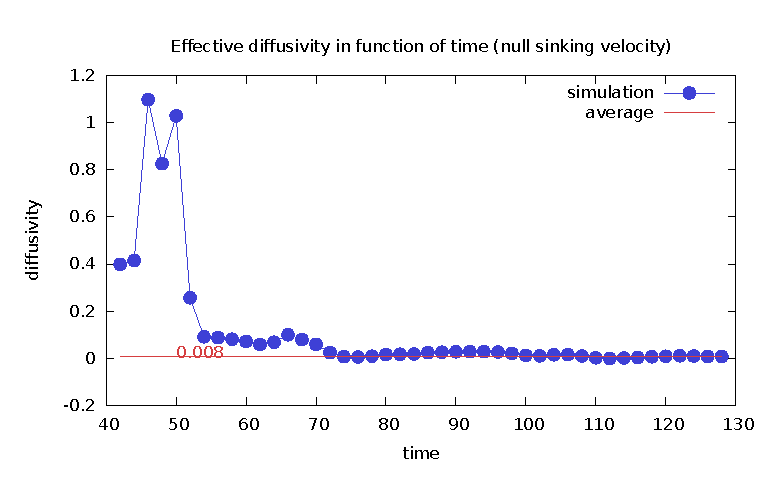
\includegraphics[width=\textwidth]{data/3D_model/run0_frequent/diffusivity}
%    \caption{Diffusivity evaluated as in \autoref{sec:taylordiff}, without reaching a steady-state.}
%    \label{fig:lag_diff_novel}
%\end{figure}

\begin{figure}[h]
        \includegraphics[width=\textwidth]{data/3D_model/run2/positions_145_1_C}
        \caption{A 3-dimensional view of the particles distribution.}
        \label{fig:lag_res_3D}
\end{figure}


\subsection{Distribution of particles} \label{sec:lag_res_distribution}


In \autoref{fig:lag_res_3D} a 3-dimensional configuration of the phytoplankton population has been plotted. In this section, the distribution over depth of the population, and its degree of non-randomness are discussed. It will turn out, as can be seen qualitatively, that there are indeed structures, not only in the vertical direction, but also horizontally.


\begin{figure}[ht]  
    \begin{subfigure}[b]{0.68\textwidth}
        \includegraphics[width=\textwidth]{data/3D_model/run2/profile_deviation}
        \caption{}
        \label{fig:lag_res_prof_deviation_profile}
    \end{subfigure}
    \begin{subfigure}[b]{0.3\textwidth}
        \begin{minipage}[t]{\linewidth}
        \includegraphics[width=\textwidth]{data/3D_model/run2/positions_110_coloured}
        \end{minipage} \quad
        \begin{minipage}[t]{\linewidth}
        \includegraphics[width=\textwidth]{data/3D_model/run2/positions_150_coloured}
        \end{minipage}
        \caption{}
        \label{fig:lag_res_prof_deviation_3D}
    \end{subfigure}
    \caption{In \autoref{fig:lag_res_prof_deviation_profile}: depth profile deviations from the average over time. Two times at which the profile deviates much from the average have been selected When the steady state is reached, the values oscillate around a stable value. In \autoref{fig:lag_res_prof_deviation_3D}: 3-dimensional distribution of cells for the two deviating profiles (colours match), where the palette saturates at 200, for sake of clarity, but the maximum value reaches respectively 1930 and 2154 for times 220 and 300.}
    \label{fig:lag_res_prof_deviation}
\end{figure}

\subsubsection{Depth profile} \label{sec:lag_res_profile}
Of qualitative interest is the shape of the depth profile $\rho(z_i,t_i)$ of the population: it is obtained making an histogram with the positions of the particles along the vertical axis, $z_i$ representing the value of distance from the bottom at the bin $i$, and $t_i$ being a discrete time at which the profile is considered. It is in principle time-dependent. \\
The result resembles that of \autoref{sec:stoc_res_profile}, having a peak under the surface and decaying towards the bottom. An average over time can be seen in \autoref{fig:lag_res_prof_deviation}, as well as two snapshots at specific times are compared with it. A characteristic feature is a second peak, deeper than the first one, which appears and disappears with time and may be a plume detaching from the bulk under the surface. This is coherent with the observation of plumes under the surface when looking at the 3-dimensional distribution (\autoref{fig:lag_res_prof_deviation_3D}); further analysis is however needed to confirm this hypothesis. 



Looking for a more quantitative approach to the evolution of the profile shape, in \autoref{fig:lag_res_rho_err} the profile is averaged over time
\[ \langle \rho \rangle \coloneqq \frac{\sum_{\{t_i\}} \rho(t)}{\Delta t} \]
The plot shows a reasonably small deviation from the mean, backing up the claim that the shape does not change much during the simulation.%; a further confirmation comes from considering the evolution in time of the following estimator $s$ of the error at a given time:
\[ s(t_i) = \frac{\sum_{\{z_i\}} \left| \rho(z_i,t_i) - \langle \rho \rangle(z_i) \right|}{N_{bins}} \]
%In \autoref{fig:lag_res_rho_err_time} the evolution of $s$ in time is displayed, showing a rather constant behaviour over time, randomly scattered around an average value. \\
Considering how the number of particles varies in time (see \autoref{sec:lag_res_number}) two main phases can be identified: the first one corresponds to an exponential growth, while the second one is a dynamical equilibrium oscillating around a central value. It is interesting to look at how the shape of the profile changes between these two phases, and a graphical comparison is in \autoref{fig:lag_res_rho_comparison}: when the quasi-steady state is reached, the peak is less pronounced, with a more consistent tail. The following interpretation is proposed: when the growth is exponential, the diffusive-advective processes (flow transport and sink; see \autoref{sec:lag_part_adv}) are not fast enough to spread the peak with respect to the birth processes; when instead the self-shading effect effectively limits the population growth rate, these spreading effects can play a substantial role, resulting in a longer tail. 

\begin{figure}[ht]
    \includegraphics[width=\textwidth]{data/3D_model/run2/profile_avg_1_50_300}
    \caption{Averaged depth profile, in the steady phase.}
    \label{fig:lag_res_rho_err} \label{fig:lag_res_prof_err}
\end{figure}

\begin{figure}[h]
        \includegraphics[width=\textwidth]{data/3D_model/run2/rho_comparison}
        \caption{The average profile during and after the exponential range (see \autoref{sec:lag_res_number}).}
        \label{fig:lag_res_rho_comparison}
\end{figure}


\subsubsection{Randomnesss} \label{sec:lag_res_random}
In order to quantitatively detect the patchiness present in the spatial distribution of the cells, a meaningful quantity which can be defined is the \textit{deviation between mean and variance}, which is an estimator of the deviation from randomness. The Poisson distribution is \autocite[chapter 8.5]{loreti2006teoria}
\[ P(x;\lambda) = \frac{e^\lambda \lambda^{-x}}{x!} \]
and its mean $\mu$ and variance $\sigma^2$ are
\[ \mu = \sigma^2 = \lambda \]
This distribution models rare, random events occurrence. Evaluating the relative difference between these two values relative to the mean gives an estimate of the deviation from the Poisson distribution, and thus from randomness. \\
For an analysis of the simulated structure, the particles have been grouped in ``boxes'' of varying size, then the number of particles in each box has been sampled, and put in a histogram which looks at the distribution of the number of particles per box along the vertical direction.
The results can be seen in \autoref{fig:lag_res_random}: the binning on vertical direction is kept constant, in order to notice the horizontal clustering structure. While increasing the dimension of horizontal bins, the deviation from randomness accentuate, to reach a maximum at $\sim\frac{1}{3}$ of the simulation box size, and then decrease. When the binning is very dense, the boxes probe a length which is too small to detect structure; on the contrary, when the binning reaches a size similar to the simulation box, the irregularities are averaged out. This means that the characteristic size of the patches is comparable to the binning size of the higher curve, that is, approximately a third of the side length. 

\begin{figure}[h]
    \includegraphics[width=\textwidth]{data/3D_model/run2/dev_poisson_1}
    \caption{The relative difference between mean and variance for the particles distribution at different binnings in the horizontal directions. The deviation from Poisson's distribution increases while increasing the bin size, having a maximum at $\sim\frac{1}{3}$ of the simulation box and then decreasing.}
    \label{fig:lag_res_random}
\end{figure}



\subsection{Number of particles} \label{sec:lag_res_number}
In \autoref{fig:lagr_v0_k0_number} the number of cells in function of time is plotted, showing an exponential transient phase, interpreted as the phase in which the self-shading effect is not large enough to damp growth. In \autoref{fig:lagr_v0_k0_number_zoom}, this transient phase is enlarged and fitted with an exponential function, whose values are shown in \autoref{tab:fit_number}. The third value shown is the prediction for the logarithmic slope made with the following reasoning. Writing \( n(z,t) = N(t) \rho(z,t) \) one can isolate the shape $\rho$ of the profile from its integral, imposing \( \int_L \rho(z,t) \dd z \equiv 1 \) with $L$ the total length of the water column. It follows that the equation \( \partial_t n(z,t) = g(z) n(z,t) \), where the self-shading effect is neglected, thus $g$ is constant in time, becomes
\[ \partial_t N(t) = N(t) \int_L g(z) \rho(z,t) \dd z \]
having as a solution
\[ N(t) = N_0e^{ \int_L g(x) \rho(z,t) \dd z \dt } \]
which if $\rho(z,t) \sim \rho(z)$ (see \autoref{fig:lag_res_prof_err}) becomes
\[ N(t) = N_0 e^{ \langle g\rangle t} \]
where the angled brackets mean a spatial average weighted with the unitary density $\rho$.

\begin{table}
    \centering
    \begin{tabular}{ c || c c | c || c}
        interval & $A$ & $k$  &  $\langle g \rho \rangle $ & $\left| \frac{k - \langle g \rho \rangle}{\sqrt{\mathrm{var}(k)+\mathrm{var}(\langle g \rho \rangle)}} \right|$ \\
        \hline 
        %$[10,25]$ & $4800\pm100$ & $0.096\pm0.001$ & $0.12\pm0.03$ & $0.80$ \\
        %$[25,50]$ & $9000\pm100$ & $0.0754\pm0.0003$ & $0.07\pm0.02$ & $0.26$ \\
        $[10,50]$ & $8100\pm100$ & $0.0777\pm0.0003$ & $0.09\pm0.02$ & $0.61$ \\
    \end{tabular}
    \caption{The parameters resulting from a fit of \autoref{fig:lagr_v0_k0_number_zoom} with the function $Ae^{kx}$ and the estimate of $k$ as the weighted average of the growth function $g$ over the profile. The fit is made with Gnuplot (\url{http://gnuplot.info/}).. Two different intervals are considered to take into account the variability of the coefficient.}
    \label{tab:fit_number}
\end{table}

\begin{figure}[h]
    \centering  
    \begin{subfigure}[b]{\textwidth}
        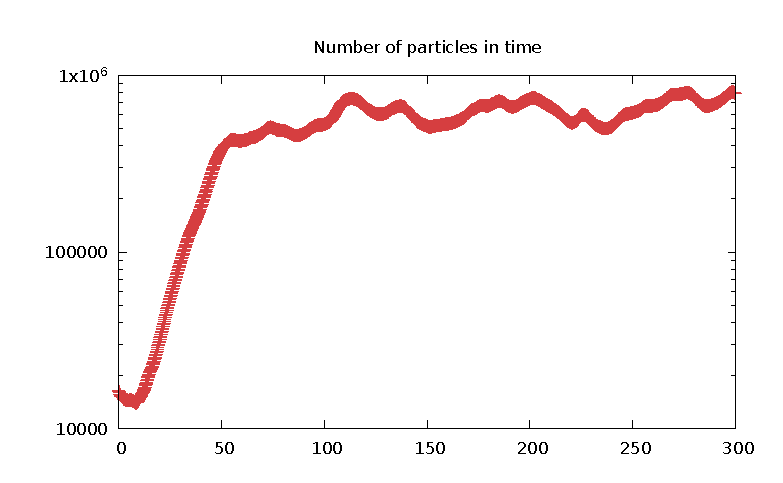
\includegraphics[width=\textwidth]{data/3D_model/run2/number_type1_log}
        \caption{}
        \label{fig:lagr_v0_k0_number}
    \end{subfigure}
    \begin{subfigure}[b]{\textwidth}
        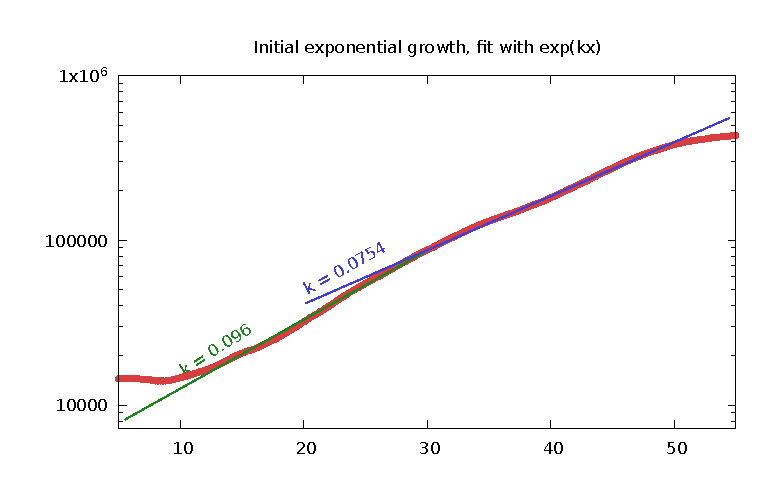
\includegraphics[width=\textwidth]{data/3D_model/run2/number_type1_log_zoom}
        \caption{}
        \label{fig:lagr_v0_k0_number_zoom}
    \end{subfigure}
    \caption{The particle number in function of time, and a closer view of the exponential growth which happens at the beginning of the simulation.}
    \label{fig:lagr_v0_k0_numbers}
\end{figure}

In \autoref{fig:lag_res_number}, the number of cells of three independent populations are plotted in function of time. The velocity changes from population to population, the other parameters being equal; this allows to measure a critical speed, defined as the average of the two higher speeds.

\begin{figure}[h]
    \includegraphics[width=\textwidth]{data/3D_model/run2/number}
    \caption{The number of particles in function of time for three different and non-interacting population. The characteristic growth time is \(\frac{1}{\mu} \sim 10\). The third type of cells is regenerated when the population dies off.}
    \label{fig:lag_res_number}
\end{figure}

\addcontentsline{toc}{chapter}{Conclusions}
\section*{Conclusions}
This work has led to the developement of two models which address the problem of predicting the phyplankton blooms. In \autoref{sec:previous}, the preexisting works have been described and systematized, providing a solid mathematical frame to the following numerical modelling. 

In \autoref{sec:stoc}, a simple stochastic model, implementing a random walk motion, has been described, which nevertheless allows to reproduce the results by \autocite{Huisman2002HowPersist} related to the subset of parameters in the D-z-v space where a bloom can occur. This model can be regarded as a fast way to explore new conditions, forerunner of a more complete analysis: beyond simulating the conditions of no-flux traditionally modeled in literature, the conditions of an absorbing bottom layer are considered and interpreted (\autoref{sec:stoc_res_abs}). \\
Trying to give some physical correspondences to the results, some cases are considered:
\begin{description}
    \item[Shallow waters] They are modeled with no-flux boundary conditions and small values of $z$. Blooming is always possible.
    \item[Mixed layer] For a well-mixed layer, the no-flux conditions offer a good description. If the depth of the ML is sufficiently large, only for intermediate values of $D$ the blooming is possible.
    \item[Deep waters] When the no-flux conditions are no more an acceptable deal, absorbing conditions must be imposed. For example, supposing to have a very shallow ML, the small-$z$ side of \autoref{fig:stoc_refl_all_pop} tells that no bloom is possible; for very deep ML, instead, the blooming conditions are equivalent to those obtained imposing no-flux boundaries.
\end{description}

In \autoref{sec:lag}, a more complete model has been tested and used to better describe the features of the plankton distribution in blooming conditions. A Lagrangian approach, which solves the Navier-Stokes equation with a pseudo-spectral method (\autoref{sec:pseudospectral}), has allowed a more complete understanding of how the particles distribute in space (\autoref{sec:lag_res_profile}, \autoref{sec:lag_res_random}) and how the growth in number is coherent with the light availability (\autoref{sec:lag_res_number}). 

Further work will concern the competition for light between two or more phytoplankton populations, in order to reproduce the results in \autocite{Huisman2004ChangesSpecies} and consider more complex settings.
\section*{Credits and aknowledgments}
\addcontentsline{toc}{section}{Credits and aknowledgments}

The pseudo-spectral code described in \autoref{sec:pseudospectral} is by Filippo De Lillo, Guido Boffetta, Matteo Borgnino \textit{et al.} from Università degli Studi di Torino. \\
Gnuplot (\url{http://gnuplot.info/}) is the tool used to plot and fit data. Some of the palettes used for the plots are from \url{https://github.com/Gnuplotting/gnuplot-palettes}. I wish to thank the site \url{http://www.gnuplotting.org} for the reference. \\
This work would have been much harder without the help by the site \url{stackoverflow.com}, my gratitude to the online coding community. \\
I wish to thank my supervisors and the other people from the research team, for their support and kindness.\\
I express my gratitude to all my friends and above all to my family, I would not be here without them.\\
Finally, if the reader does not belong to any of the groups above, thanks to him for having got to the end.
\appendix
%\subsection{Random number generator} \label{subsec:rng}
%By G. Boffetta. rann, gaus
\chapter{Numerical methods}
\section[Runge-Kutta]{Runge-Kutta algorithms}
Runge-Kutta (RK) algorithms are a family of algorithms designed to solve ordinary differential equations of the form
\[ y' \coloneqq \frac{\dd y(t)}{\dt} = f(t,y(t)) \]
The exact solution of the problem is \(y_n=y(t_n)\) where \( t_n = t_0+n\mathrm{d}t\) is the discretized time; instead, \(u_n\) is the solution obtained with the algorithm. The reference for this section is \autocite{quarteroni2010numerical}
A RK algorithm is defined as follows: 
\[ u_{n+1} = u_n + h \sum_{i=1}^s b_i K_i\]
where
\begin{equation} \label{eq:RK_Ki} 
    K_i = f(t_n+c_i h, u_n+h \sum_{j=1}^s a_{ij} K_j)
\end{equation}
and
\begin{equation} \label{eq:RK_ci}
    c_i = \sum_{j=1}^s a_{ij} 
\end{equation}
It is clear from \autoref{eq:RK_Ki} that the $K_i$ are in principle defined implicitly (i.e. a linear system must be solved in order to find them); however, imposing the condition that \( a_{ij} = 0 \) for \( j\geq i\) makes the system \textit{explicit}, since using \autoref{eq:RK_ci}  
\[ K_1 = f(t_n,u_n) \]
which is known, $K_2$ is function of $K_1$ only, $K_3$ is function of $K_2$ and $K_1$ and so on, such that no matrix inversion is necessary.

The number $s$ is said to be the number of \textit{stages} of a RK algorithm. For an explicit algorithm, 
\begin{quotation}
The order of an $s$-stage explicit RK method cannot be greater than $s$. Also, there do not exist $s$-stage explicit RK methods with order $s$ if $s \geq 5$.
\end{quotation}


\subsection{Derivation of RK2 algorithm}
Given a $s$-stage RK algorithm, one can tune the parameter to make it of order equal to that of the algorithm be $s$ (or $s+1$, for $s>4$) by Taylor-expanding $u_{n+1}$ and $y_{n+1}$ until order $s-1$ and imposing that the coefficient be the equal. The procedure can be illustrated deriving a second-order RK algorithm (RK2).

Since the $K_i$ system is explicit, using \autoref{eq:RK_ci}
\[ K_1 = f_n \]
and 
\[ K_2 = f(t_n+hc_2, u_n + h c_2 f_n) \]
Following the notation in \autocite[chapter 11.8]{quarteroni2010numerical}, 
\[ f_n \coloneqq f(t_n,u_n) \equiv f(t_n,y_n) \;\;;\;\;\; f_{n,t} \coloneqq \frac{\partial f}{\partial t}|_{(t_n,y_n)} \;\;;\;\;\;
f_{n,y} \coloneqq \frac{\partial f}{\partial y}|_{(t_n,y_n)}\]
Expanding near $f_n$

\[ K_2 \sim f_n + h c_2 (f_{n,t} + f_nf_{n,y}) + \mathcal{O}(h^2) \]
so that
\[ u_{n+1} = u_n + h(b_1K_1 + b_2K_2) \]
\[   = u_n + hb_1 f_n + b_2 h^2 c_2 (f_{n,t} + f_n f_{n,y} ) \]
while for the exact solution
\[ y_{n+1} = y_n + hy_n' +\frac{h^2}{2}y_n'' +\mathcal{O}(h^3) \]
\[  = y_n + h f_n + \frac{h^2}{2} (f_{n,t} + y_n' f_{n,y}) \]
\[ = y_n + h f_n + \frac{h^2}{2} (f_{n,t} + f_n f_{n,y}) \]
and matching the coefficients the following conditions are derived:
\begin{equation}
    \begin{cases}
        b_1+b_2 = 1 & \\
        b_2c_2 = \frac{1}{2} & \\
    \end{cases}
\end{equation}
In particular, choosing 
\[ b_1 = -1 \;\;;\;\;\; b_2 = 1 \;\;;\;\;\; c_2 = \frac{1}{2} \]
it results
\begin{equation} \label{eq:RK2}
u_{n+1} = u_n + \frac{h}{2} f(t_n + \frac{h}{2},
u_n + \frac{h}{2} f_n) 
\end{equation}
Defining
\begin{equation}
    \begin{cases}
        t_{n+1/2} \coloneqq t_n + \frac{h}{2} & \\
        u_{n+1/2} \coloneqq u_n + \frac{h}{2} f_n  & \\
    \end{cases}
\end{equation}
\autoref{eq:RK2} can be rewritten as
\begin{equation} \label{eq:RK2_halfstep}
    u_{n+1} = u_n + \frac{h}{2} f(t_{n+1/2},u_{n+1/2})
\end{equation}


 
\chapter{Testing}
\section{Stochastic model}
\subsection{Birth rate} \label{sec:model:birthrate}
In order to evaluate the birth rate at a given depth, the following equation models a production process which saturates (see \autoref{sec:math-model}):
\begin{equation}
  f(z,t) = \lambda \frac{I(z,t)}{H + I(z,t)}
\end{equation}
where
\[ I(z,t) = e^{-k_{bg}z-k_{ss}\int_0^z n(z,t)} \]
Converting this equation to a discrete context, at a given time, for a given particle $i$
\[ I(i) = e^{-k_{bg}z_i - k_{ss}\sum_{\{\hat{j}\}}1} \]
where $\hat{j}$ represents the indexes of particles which are at a shallower depth than the one labelled with $i$.
However, this exact method of summing the particles is computationally expensive, since one has to nest two loops over the particles: the inner one increments the value of the sum with the condition above, while the outer one assigns this value to the $i$th cell, resulting in a $\mathcal{O}(N^2)$ operation. A much faster way to approach this is to fill a histogram with the cells, then sum incrementally over the bins in order to get the value of the sum on a discrete set of points; now it is possible to assign the birth rates either choosing the upper (or lower) value on the grid, or interpolating with the following linear espression:
\[ f(x) \simeq (x_2-x)f(x_1)+(x-x_1)f(x_2) \]
Some comparisons are shown in \autoref{fig:compare_integral}, from a simulation run with 1000 cells: an error has to be expected due to the approximation, but for the most part of the points it is below 10\%; even better when considering the estimate of the birth rate, where the errors are well below 1\%. Considering that the birth rate is actually the interesting quantity, the approximation is acceptable and it has been used instead of the exact method in order to make the code faster.

\begin{figure}
 \begin{subfigure}[b]{0.45\textwidth}
    \includegraphics[width=\textwidth]{data/1D_model/test_integral/interpolated_integral}
    \caption{}
    \label{fig:interpolated_integral}
  \end{subfigure}
  %add desired spacing between images, e. g. ~, \quad, \qquad, \hfill etc. 
  %(or a blank line to force the subfigure onto a new line)
  \begin{subfigure}[b]{0.45\textwidth}
    \includegraphics[width=\textwidth]{data/1D_model/test_integral/interpolated_preproduction}
    \caption{}
    \label{fig:interpolated_preproduction}
  \end{subfigure}
  \caption{Comparison between the exact and interpolated methods described in \autoref{sec:model:birthrate}. In \autoref{fig:interpolated_integral} the interpolated integral is shown for each particle in the simulation, with an inset concerning the relative deviations from the exact integral; in \autoref{fig:interpolated_preproduction}, the same is made for the reproduction rate.}
  \label{fig:compare_integral}
\end{figure}



\subsection{No-flux conditions} \label{sec:no-flux-test}

In this numerical model, the following implementation for the boundary conditions has been used, where \(x' = v \mathrm{d}t + \sqrt{2D\cdot \mathrm{d}t}\zeta\) as in \autoref{eq:eul-difadv}:
\begin{equation}
x_i^{n+1} = \begin{cases}
    x' &\mathrm{if}\; x' \in [x_{min},x_{max}] \\
    2x_{min} - x' &\mathrm{if}\; x' < x_{min} \\
    2x_{max} - x' &\mathrm{if}\; x' > x_{max} 
\end{cases}
\end{equation}

\paragraph{Validation}
In order to validate the model, some testing is performed about no-flux conditions.
The one-dimensional diffusion-advection equation
\begin{equation} \label{eq:n-difadv}
  \partial_t n(x,t) = -v\partial_x n(x,t) +D\partial^2_x n(x,t) 
\end{equation}
is considered: $n$ represents a density of particles, diffused with a coefficient $D$ and advected towards biggest values of $x$ (for positive values of $v$). This equation relates to the 1-dimensional phytoplankton model by imposing both the production and loss factors to 0. An analytic solution can be derived for closed boundaries: defining the current \( J := vn - D\partial_x n \), 
the no-flux conditions at a point $\bar{x}$ can be written as (\autocite{Huisman2002HowPersist})
\begin{equation} \label{eq:noflux}
J(\bar{x}) = 0
\end{equation}
and \autoref{eq:n-difadv} becomes
\[ \partial_t n + \partial_x J = 0 \]
The following steady-state condition holds:
\[ \partial_x J = 0 \]
Defining the auxiliary variable \( \xi=\xi\partial_xn \) a solution is 
\[ \xi(x) = \xi_0 e^{\frac{v(x-x_0)}{D}} \]
where $x_0$ is the lowest value of $x$; this gives
\[ n(x) = \xi_0 \frac{D}{v} e^{\frac{v(x-x_0)}{D}} + n_0 \;\;. \]
and 
\[ J(x) = v n_0 = const \]
Imposing no-flux conditions means 
\[ J(x_0) = vn_0 = 0 \;\; \Rightarrow \;\; n_0 = 0\]
so the general solution with no-flux boundaries is
\begin{equation} \label{eq:rho-noflux-da}
  n(x) = \alpha \frac{D}{v} e^{\frac{v(x-x_0)}{D}} \;\;.
\end{equation}
where $\alpha$ is a constant depending on the initial conditions.
A formula for this constant can be obtained evaluating the number of particles
\[ N(x) = \int_{x_0}^{x} n(x) \mathrm{d}x = \alpha \frac{D}{v} \left( e^{\frac{v(x-x_0)}{D}} - 1 \right) \]
which gives
\begin{equation} \label{eq:rho-noflux-const}
  \alpha =\frac{N(x)}{\left(\frac{D}{v}\right)^2\left( e^{\frac{v(x-x_0)}{D}} - 1 \right)}
\end{equation}

% The Eulerian integration is performed in an interval \( [0,1] \), where $10^5$ particles are uniformly distributed at time zero (since we are looking for a stationary solution, this detail is not influent). The parameters used in the simulation are listed in \autoref{tab:eul-par}.
This analytic result serves as a test distribution which has to be matched by the model developed. 
\autoref{eq:rho-noflux-const} with the parameters in \autoref{tab:eul-par}, used for the simulation, becomes 
\[ \alpha = \frac{1}{(e-1)n_{bin}} \]
where $n_{bin}$ is the number of bins of the histogram, introduced because of the normalization. \\
As can be seen in \autoref{img:bound-refl-fit}, the fit is good, thus confirming that the chosen implementation of no-flux conditions is consistent.

\begin{table} 
  \begin{center}
    \begin{tabular}{ c | c | c | c} 
      \hline
      D               & v             & $z_0$    & $z_{max}$ \\ \hline
      $0.01m^2h^{-1}$ & $0.01mh^{-1}$ & $0m$     & $1m$        \\
      \hline
    \end{tabular}
  \end{center}
  \caption{Parameters used for the simulation of \autoref{eq:eul-difadv}. }
  \label{tab:eul-par}
\end{table}

\begin{figure}[!htb]
  \centering
  \begin{subfigure}[b]{0.4\textwidth}
    \includegraphics[width=1\textwidth]{data/1D_model/reflective_bottom/noflux_conditions/cfr_stoc_refl}
    \caption{}
    \label{img:bound-refl-fit}
  \end{subfigure}
  \begin{subfigure}[b]{0.4\textwidth}
    \includegraphics[width=1\textwidth]{data/1D_model/reflective_bottom/noflux_conditions/cfr_stoc_refl_residuals}
    \caption{}
    \label{img:bound-refl-fit-residuals}
  \end{subfigure}
  \caption{In \autoref{img:bound-refl-fit} the fit is shown of the distribution of particles averaged near equilibrium, according to \autoref{eq:eul-difadv}, with parameters in \autoref{tab:eul-par}. 
  In \autoref{img:bound-refl-fit-residuals} the residuals of the actual distribution with respect to the analytic one are plotted.
  Simulation run with $2500$ particles.}
\end{figure}

\section{Lagrangian model}
In order to check the consistence of the numerical model with expected results, some tests are performed.

%\subsection{Sinking velocity}
%The Lagrangian code is modified in order to nullify the effects of advective flow and reactions of the cells. Since $dt=5\cdot10^{-3}$ and $v=1$, after $1000$ iterations the particles are expected to have travelled $5$.


\subsection{Light intensity}
%Run with (make copies of files):
%\begin{itemize}
%    \item initial random particle distribution
%    \item position does not evolve (use no\_advection)
%    \item $\lambda=0$, $\mu=0$
%    \item in popul.f90 write $(x_{particle},intens)$
%    \item look at "denso.xxx"
%\end{itemize}
%Profile should be exponential (integral over depth is linear) and in 0 should be =1.
In particular, since the distribution here is uniform, given $N$ total particles it will result \( \int_0^z n(r) \mathrm{d}r \sim \int_0^z \frac{N}{L_z} \mathrm{d}r = z\frac{N}{L_z} \) so that, following \autoref{eq:generic_light},
\begin{equation} \label{eq:light_func}
    \frac{I(z)}{I_0} \sim e^{-z(k_{bg}+k_{ss}\frac{N}{L_z})} 
\end{equation}
The numerical results are compared with these analytical results in \autoref{fig:3d:light_profile}; the residuals are shown in \autoref{fig:3d:light_residuals} and, normalized, in \autoref{fig:3d:light_residuals_relative}; the light as perceived by the particles is plotted in \autoref{fig:3d:light_seen_particles}.

\begin{figure} 
  \centering
  \begin{subfigure}[b]{\textwidth}
    \includegraphics[width=\textwidth]{data/3D_model/light_profile}
    \caption{}
    \label{fig:3d:light_profile}
  \end{subfigure}
  \begin{subfigure}[b]{\textwidth}
    \includegraphics[width=\textwidth]{data/3D_model/light_seen_particle}
    \caption{}
    \label{fig:3d:light_seen_particles}
  \end{subfigure}
    \caption{In \autoref{fig:3d:light_profile} the light intensity set at grid-points is plotted against the theoretical function \autoref{eq:light_func} (see \autoref{sec:ref_crit_turb}); in \autoref{fig:3d:light_seen_particles} the light intensity as seen by each particle is plotted in function of their position.}
    \label{fig:3d_light_A}
\end{figure}
\begin{figure} 
  \centering
  \begin{subfigure}[b]{\textwidth}
    \includegraphics[width=\textwidth]{data/3D_model/light_residuals}
    \caption{}
    \label{fig:3d:light_residuals}
  \end{subfigure}
  
  \begin{subfigure}[b]{\textwidth}
    \includegraphics[width=\textwidth]{data/3D_model/light_residuals_relative}
    \caption{}
    \label{fig:3d:light_residuals_relative}
  \end{subfigure}
  \caption{The residuals are shown of light intensity with respect to the theoretical function \autoref{eq:light_func} (see \autoref{fig:3d:light_profile}): in \autoref{fig:3d:light_residuals} the simple difference is considered, while in \autoref{fig:3d:light_residuals_relative} a normalization on by the intensity value has been made.}
    \label{fig:3d_light_B}
\end{figure}


\subsection{Growth reaction}
Modifying the code to eliminate transport both by advective flow and sinking velocity, an exponential growth should be seen if $k_as$ (the auto-shading parameter) is set to zero. The modeling equation is (see \autoref{eq:n-difadv})
\[ \partial_t n(t,z) = \left(\frac{\lambda}{1+\frac{h}{I_0}e^{k_{bg}z}} -\mu\right)n(t,z) = f(z)n(t,z)\]
so the resulting numerical density at a depth $z$ is
\[ n(t,z) = n(0,z)e^{f(z)t} . \]


  
%\input{tex/appendices/notes}                




\addcontentsline{toc}{chapter}{Bibliography}
\printbibliography
\addcontentsline{toc}{chapter}{List of Figures}
\listoffigures



\end{document}
